%    PACKAGES AND THEMES
%----------------------------------------------------------------------------------------

\documentclass[aspectratio=169,xcolor=dvipsnames]{beamer}
\usetheme{SimpleDarkBlue}

\usepackage{hyperref}
\usepackage{graphicx} % Allows including images
\usepackage{booktabs} % Allows the use of \toprule, \midrule and \bottomrule in tables
\usepackage{subcaption} 
\usepackage{tikz}
\usepackage{natbib}

\usepackage[normalem]{ulem}

\usetikzlibrary{arrows.meta, positioning, shapes, calc, decorations.pathreplacing}

%----------------------------------------------------------------------------------------
%    TITLE PAGE
%----------------------------------------------------------------------------------------

\title{Minimization of Maximum Mean Discrepancy (MMD)}
\author{Zonghao (Hudson) Chen}

\date[]{}
% Date, can be changed to a custom date

\usepackage{amsthm}
\newtheorem{thm}{Theorem}
\newtheorem*{thm*}{Theorem}
\newtheorem{cor}[theorem]{Corollary}
\newtheorem{lem}[theorem]{Lemma}
\newtheorem{prop}[theorem]{Proposition}
\newtheorem*{prop*}{Proposition}
\newtheorem{rem}[theorem]{Remark}
\newtheorem{defi}{Definition}
\newtheorem{ass}{Assumption}



\definecolor{definitionTitle}{RGB}{34, 102, 102}  % A deep teal color
\definecolor{definitionBody}{RGB}{10, 10, 10}     % Near-black for text
\definecolor{mmdGreen}{RGB}{46, 125, 50}
\definecolor{mmdBlue}{RGB}{25, 96, 170}
\definecolor{mmdRed}{RGB}{180, 70, 55}
\definecolor{answerBody}{RGB}{225, 244, 244}

\setbeamercolor{block title alerted}{bg=brown, fg=white}
\setbeamercolor{block body alerted}{fg=definitionBody}
\setbeamercolor{answer box}{bg=answerBody, fg=black}

% Now redefine the 'defi' environment to use the 'alerted block' style:
\setbeamertemplate{theorems}[numbered]
\let\olddefi\defi
\renewenvironment{defi}[1][]{%
  \begin{alertblock}{Definition\ifx\\#1\\\else~(#1)\fi}%
}{%
  \end{alertblock}%
}

\newenvironment{answerblock}{%
  \begin{beamercolorbox}[wd=\linewidth, sep=0.15em, rounded=true, shadow=true]{answer box}%
}{%
  \end{beamercolorbox}%
}

\definecolor{graytext}{gray}{0.5} % Customize the grey level if needed
% Save the original versions
\let\oldcitep\citep
\let\oldcitet\citet

% Render slide citations as compact grey alphabetic labels.
\renewcommand{\citep}[1]{{\scriptsize\textcolor{graytext}{\oldcitep{#1}}}}
\renewcommand{\citet}[1]{{\scriptsize\textcolor{graytext}{\oldcitet{#1}}}}
\renewcommand{\cite}[1]{{\scriptsize\textcolor{graytext}{\oldcitep{#1}}}}
\newcommand{\red}[1]{\textcolor{red}{#1}}
\newcommand{\green}[1]{\textcolor{green!60!black}{#1}}
\newcommand{\orange}[1]{\textcolor{orange}{#1}}
\newcommand{\blue}[1]{\textcolor{blue}{#1}}
\newcommand{\mmdicon}[2]{%
    \tikz[baseline=(icon.base)]{
        \node[circle, fill=#1, text=white, inner sep=1.2pt, font=\scriptsize\bfseries] (icon) {#2};
    }%
}
\newcommand{\bookicon}[1]{%
    \tikz[baseline=-0.5ex, scale=0.18]{
        \fill[#1!18] (0,0) rectangle (1.55,1.75);
        \fill[#1!28] (1.55,0) rectangle (3.1,1.75);
        \draw[#1!80!black, line width=0.45pt, rounded corners=0.4pt]
            (0,0) rectangle (1.55,1.75)
            (1.55,0) rectangle (3.1,1.75);
        \draw[#1!80!black, line width=0.45pt] (1.55,0) -- (1.55,1.75);
        \draw[#1!70!black, line width=0.3pt] (0.35,1.25) -- (1.18,1.25);
        \draw[#1!70!black, line width=0.3pt] (1.92,1.25) -- (2.75,1.25);
        \draw[#1!70!black, line width=0.3pt] (0.35,0.85) -- (1.18,0.85);
        \draw[#1!70!black, line width=0.3pt] (1.92,0.85) -- (2.75,0.85);
    }%
}
\newcommand{\parttitleframe}[1]{%
    \begin{frame}[plain]
        \centering
        \vfill
        {\Huge\bfseries #1}
        \vfill
    \end{frame}
}

\newenvironment{talign*}
 {\let\displaystyle\textstyle\csname align*\endcsname}
 {\endalign}
\newenvironment{talign}
 {\let\displaystyle\textstyle\csname align\endcsname}
 {\endalign}
 
%----------------------------------------------------------------------------------------
%    PRESENTATION SLIDES
%----------------------------------------------------------------------------------------

\begin{document}

\newcommand{\E}{\mathbb{E}}
\newcommand{\R}{\mathbb{R}}
\newcommand{\Qb}{\mathbb{Q}}
\newcommand{\Pb}{\mathbb{P}}
\newcommand{\calH}{\mathcal{H}}
\newcommand{\calN}{\mathcal{N}}
\newcommand{\calM}{\mathcal{M}}
\newcommand{\calE}{\mathcal{E}}
\newcommand{\calT}{\mathcal{T}}
\newcommand{\calL}{\mathcal{L}}
\newcommand{\calF}{\mathcal{F}}
\newcommand{\calG}{\mathcal{G}}
\newcommand{\calZ}{\mathcal{Z}}
\newcommand{\calO}{\mathcal{O}}
\newcommand{\calX}{\mathcal{X}}
\newcommand{\calP}{\mathcal{P}}
\newcommand{\dd}{\mathrm{d}}
\newcommand{\bx}{\mathbf{x}}
\newcommand{\bo}{\mathbf{o}}
\newcommand{\by}{\mathbf{y}}
\newcommand{\bz}{\mathbf{z}}
\newcommand{\bH}{\mathbf{H}}
\newcommand{\bw}{\mathbf{w}}
\newcommand{\bJ}{\mathbf{J}}
\newcommand{\bnabla}{\boldsymbol{\nabla}}
\newcommand{\scrG}{\mathscr{G}}
\newcommand{\scrF}{\mathscr{F}}
\newcommand{\scrX}{\mathscr{X}}
\newcommand{\scrx}{\mathscr{X}}
\newcommand{\scrY}{\mathscr{Y}}
\newcommand{\scry}{\mathscr{Y}}
\newcommand{\scrZ}{\mathscr{Z}}
\newcommand{\scrz}{\mathscr{Z}}
\newcommand{\scrU}{\mathscr{U}}
\newcommand{\scrR}{\mathscr{R}}
\newcommand{\scrQ}{\mathscr{Q}}
\newcommand{\scrL}{\mathscr{L}}

\newcommand{\Id}{\mathrm{Id}}
\newcommand{\N}{\mathbb{N}}
\newcommand{\kl}{\mathrm{KL}}
\newcommand{\tv}{\mathrm{TV}}
\newcommand{\LSI}{\mathrm{LSI}}
\newcommand{\mmd}{\mathrm{MMD}}
\newcommand{\dmmd}{\mathrm{DrMMD}}

\newcommand{\one}{\mathbf{1}}


\begin{frame}
    % Print the title page as the first slide
    \titlepage
    \vspace{-1.5cm}
    \begin{center}
        % \textit{Annual student conference, UCL Computer Science, 2026} 
    \end{center}
\end{frame}




\section{Personal}
\begin{frame}{About Me}
    \vspace{-0.25cm}
    \begin{columns}[T,onlytextwidth]
        \column{0.34\textwidth}
        \begin{minipage}[t][0.68\textheight][t]{\linewidth}
            \centering
            \begin{tikzpicture}
                \node[
                    draw=mmdBlue!55!black,
                    line width=0.8pt,
                    rounded corners=4pt,
                    inner sep=2.5pt
                ] {
                    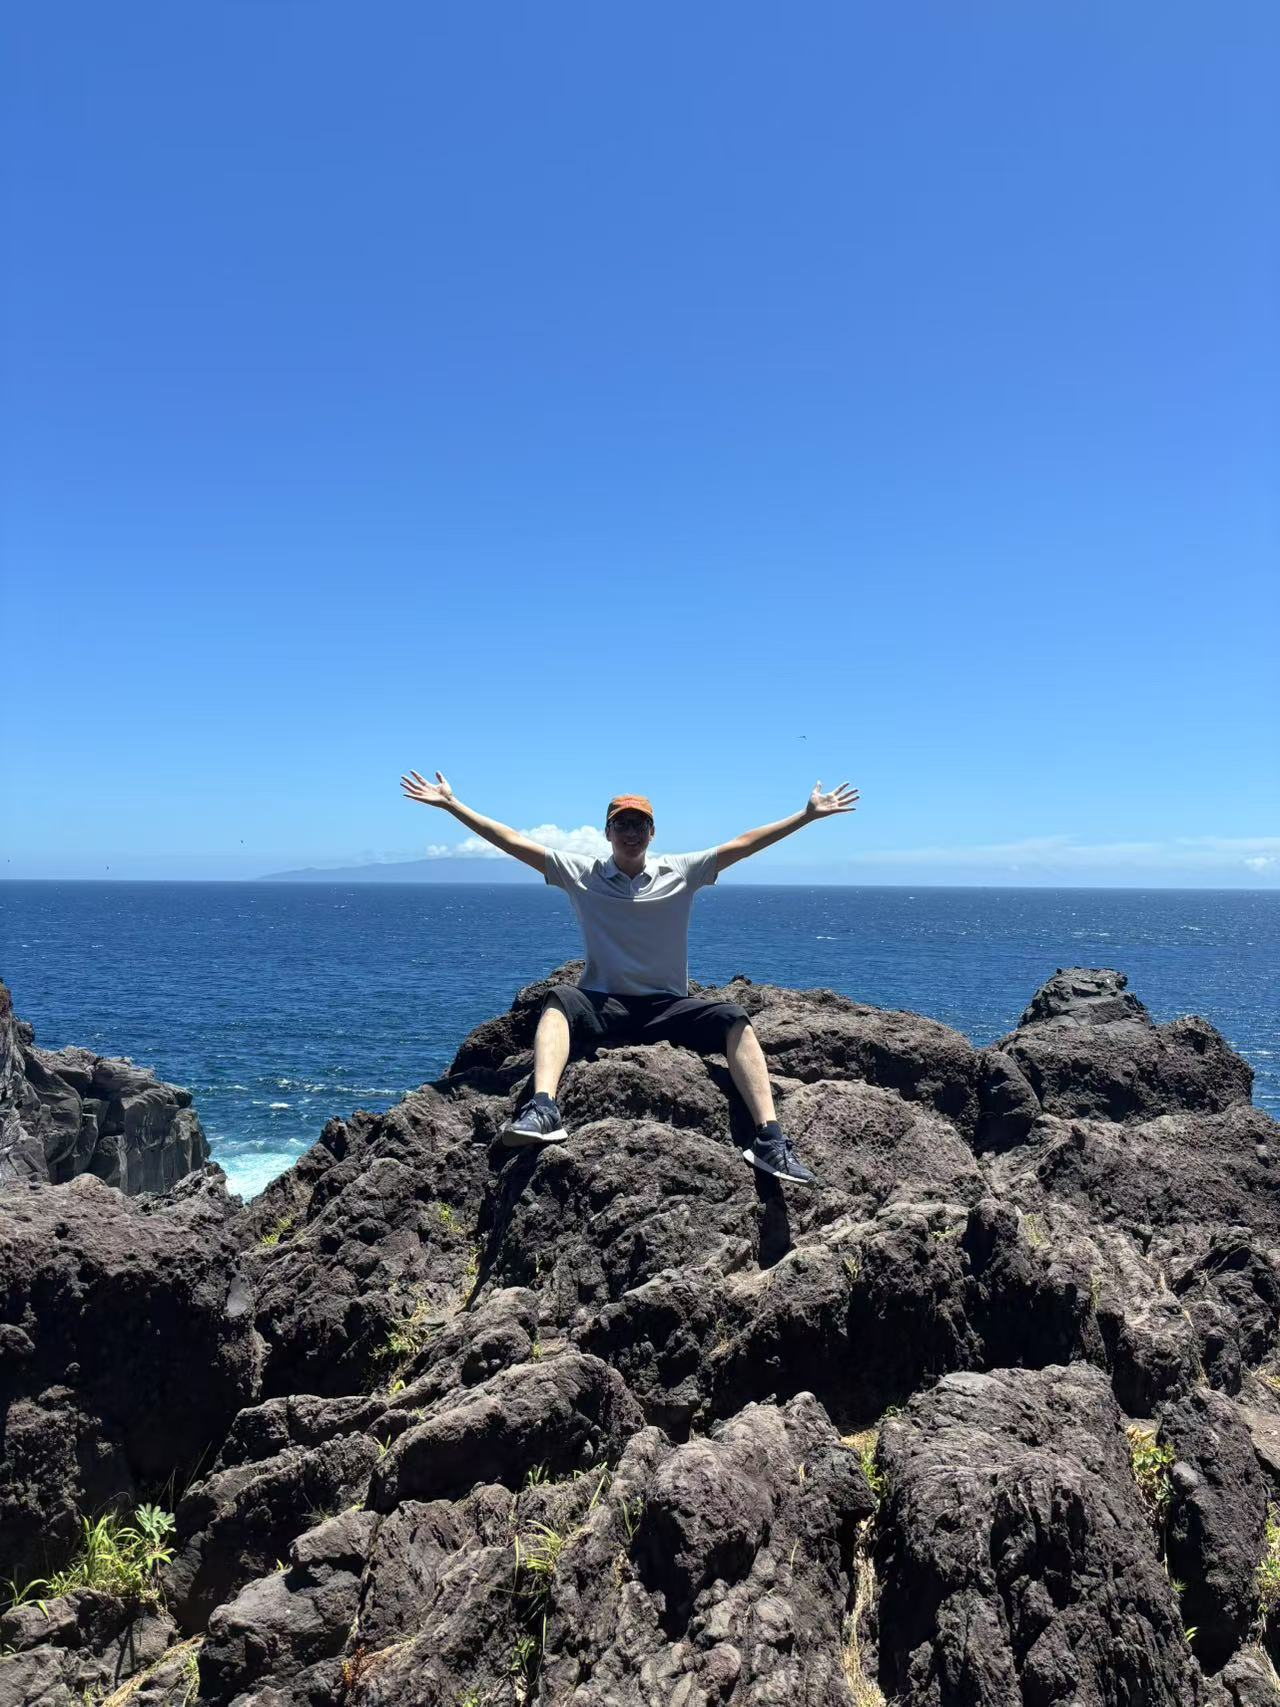
\includegraphics[width=0.86\linewidth,height=0.58\textheight,keepaspectratio]{figures/personal.png}
                };
            \end{tikzpicture}
        \end{minipage}

        \column{0.62\textwidth}
        {\Large\bfseries Zonghao (Hudson) Chen}\\[-0.04cm]
        {\small\color{graytext}4th year PhD student, University College London}\\[0.22cm]

        \begin{beamercolorbox}[wd=\linewidth, sep=0.33em, rounded=true]{answer box}
            \small
            \begin{tabular}{@{}p{0.44\linewidth}p{0.46\linewidth}@{}}
                Foundational AI Centre & Fran\c{c}ois-Xavier Briol\\
                Gatsby Unit & Arthur Gretton
            \end{tabular}
        \end{beamercolorbox}

        \vspace{0.18cm}
        \begin{beamercolorbox}[wd=\linewidth, sep=0.33em, rounded=true]{answer box}
            \small
            Tsinghua Uni., B.Eng. in Electronic Engineering, 2022
        \end{beamercolorbox}

        \vspace{0.18cm}
        \begin{beamercolorbox}[wd=\linewidth, sep=0.33em, rounded=true]{answer box}
            {\bfseries Research Interests}\\
            \small
            \vspace{-0.14cm}
            \begin{itemize}
                \setlength\topsep{0pt}
                \setlength\partopsep{0pt}
                \setlength\parsep{0pt}
                \setlength\itemsep{0.02cm}
                \item Kernel and nonparametric methods
                \item Causal inference
                \item Statistical learning theory
            \end{itemize}
            \vspace{-0.26cm}
        \end{beamercolorbox}
    \end{columns}
\end{frame}

\section{Content}
\begin{frame}{Research timeline}
    \centering
    {\large\bfseries A research timeline from the start of my PhD}\\[0.28cm]

    \begin{tikzpicture}[
        x=1cm,
        y=1cm,
        timeline/.style={line width=1.2pt, -{Latex[length=2.4mm]}, mmdBlue!75!black},
        tick/.style={mmdBlue!75!black, line width=0.8pt},
        eventBase/.style={
            rounded corners=2pt,
            line width=0.7pt,
            text width=3.0cm,
            align=center,
            inner sep=4pt,
            font=\scriptsize
        },
        eventBlue/.style={eventBase, draw=mmdBlue!75!black, fill=mmdBlue!8},
        eventGreen/.style={eventBase, draw=mmdGreen!75!black, fill=mmdGreen!8},
        eventRed/.style={eventBase, draw=mmdRed!75!black, fill=mmdRed!8},
        dotBlue/.style={circle, fill=mmdBlue!80!black, draw=white, line width=0.5pt, minimum size=5pt, inner sep=0pt},
        dotGreen/.style={circle, fill=mmdGreen!80!black, draw=white, line width=0.5pt, minimum size=5pt, inner sep=0pt},
        dotRed/.style={circle, fill=mmdRed!80!black, draw=white, line width=0.5pt, minimum size=5pt, inner sep=0pt}
    ]
        \draw[timeline] (0,0) -- (11.6,0);

        \foreach \x/\label in {0/{09/2022},2.1/{2023},4.4/{2024},7.1/{2025},9.7/{2026}} {
            \draw[tick] (\x,0.12) -- (\x,-0.12);
            \node[font=\scriptsize, text=mmdBlue!80!black] at (\x,-0.42) {\label};
        }

        \node[dotBlue] at (0,0) {};
        \node[eventBlue, text width=2.35cm] (phdstart) at (0,1.15)
            {\bfseries PhD starts\\[-0.02cm]
             \textcolor{graytext}{UCL, Sep 2022}};
        \draw[mmdBlue!60!black, line width=0.6pt] (0,0.08) -- (phdstart.south);

        \node[dotGreen] at (2.6,0) {};
        \node[eventGreen] (integration) at (2.6,-1.10)
            {\bfseries Kernel-based\\
             numerical integration};
        \draw[mmdGreen!60!black, line width=0.6pt] (2.6,-0.08) -- (integration.north);

        \node[dotBlue] at (5.7,0) {};
        \node[eventBlue] (sampling) at (5.7,1.28)
            {\bfseries Sampling / Generative\\
             modelling via MMD flows};
        \draw[mmdBlue!60!black, line width=0.6pt] (5.7,0.08) -- (sampling.south);

        \node[dotRed] at (8.8,0) {};
        \node[eventRed] (inference) at (8.8,-1.32)
            {\bfseries Minimum MMD estimators\\
             for inference};
        \draw[mmdRed!60!black, line width=0.6pt] (8.8,-0.08) -- (inference.north);

        \node[font=\scriptsize\bfseries, text=mmdBlue!80!black, align=center] at (11.25,0.48)
            {Today};

        \draw[
            decorate,
            decoration={brace, mirror, amplitude=8pt},
            line width=1.1pt,
            mmdBlue!80!black
        ] (1.25,-1.95) -- (10.15,-1.95)
            node[midway, yshift=-0.62cm, font=\large\bfseries, text=mmdBlue!85!black]
            {Minimization of Maximum Mean Discrepancy (MMD)};
    \end{tikzpicture}
\end{frame}

\begin{frame}{Background: what is MMD?}
    \begin{columns}[c]
        \column{0.50\textwidth}
        \begin{itemize}
            \item Given two distributions $\Pb$ and $\Qb$, how to compare them? 
            \item Compute the difference of their means: $|\E_{\Pb}[X] - \E_{\Qb}[X]|$. 
            \item Compute the difference of their second moments: $|\E_{\Pb}[X^2] - \E_{\Qb}[X^2]|$.
            \item The first two moments are not enough! 
        \end{itemize}

        \column{0.5\textwidth}
        \centering
        \begin{tikzpicture}[scale=0.88, every node/.style={font=\scriptsize}]
            \draw[blue!80!black, very thick] (-0.8,2.35) -- (-0.35,2.35)
                node[right, black] {$\Pb$};
            \draw[orange!90!black, very thick] (0.55,2.35) -- (1.0,2.35)
                node[right, black] {$\Qb$};

            \fill[blue!25, opacity=0.75]
                plot[smooth, samples=100, domain=-2.7:2.0]
                (\x,{1.75*exp(-0.5*((\x+0.75)/0.72)^2)});
            \draw[blue!80!black, very thick]
                plot[smooth, samples=100, domain=-2.7:2.0]
                (\x,{1.75*exp(-0.5*((\x+0.75)/0.72)^2)});

            \fill[orange!30, opacity=0.7]
                plot[smooth, samples=100, domain=-1.2:3.1]
                (\x,{1.35*exp(-0.5*((\x-0.85)/0.95)^2)});
            \draw[orange!90!black, very thick]
                plot[smooth, samples=100, domain=-1.2:3.1]
                (\x,{1.35*exp(-0.5*((\x-0.85)/0.95)^2)});

            \draw[blue!80!black, dashed, thick] (-0.75,0) -- (-0.75,1.95)
                node[above] {mean};
            \draw[orange!90!black, dashed, thick] (0.85,0) -- (0.85,1.55)
                node[above] {mean};

        \end{tikzpicture}
    \end{columns}
    \vspace{0.3cm}
    \begin{exampleblock}{}
\centering
    \textbf{Goal}: Compare $\Pb$ and $\Qb$ with a general $f$, i.e., $|\E_{\Pb}[f(X)] - \E_{\Qb}[f(X)]|$?
\end{exampleblock}
\end{frame}

\begin{frame}{Background: Maximum Mean Discrepancy (MMD)~\citep{gretton2012kernel}}
    \begin{columns}[c]
        \column{0.8\textwidth}
        \begin{itemize}
            \item $\calH$ is a reproducing kernel Hilbert space (RKHS) with kernel $k$.
            \begin{align*}
                \text{MMD}(\Pb, \Qb)
                := \sup_{f \in \calH}
                |\E_{\Pb}[f(X)] - \E_{\Qb}[f(X)]|.
            \end{align*}
            \item The RKHS contains functions that are linear combinations of the feature maps $\phi:\calX\to\calH$, $f=\sum_{i=1}^n \alpha_i \phi(x_i)$.

        \end{itemize}

        \column{0.2\textwidth}
        \centering
        \begin{tikzpicture}[scale=0.72, every node/.style={font=\scriptsize}]
            \begin{scope}
                \draw[->, thick] (-1.55,0) -- (1.75,0) node[right] {$x$};
                \node[above] at (0.1,0.38) {input space};

                \foreach \x in {-0.9,-0.65,-0.35,-0.1} {
                    \fill[blue!80!black] (\x,0) circle (2pt);
                }
                \foreach \x in {0.45,0.7,1.0,1.25} {
                    \fill[orange!90!black] (\x,0) circle (2pt);
                }
                \node[blue!80!black] at (-0.55,-0.35) {$\Pb$};
                \node[orange!90!black] at (0.95,-0.35) {$\Qb$};
            \end{scope}
            \vspace{0.2cm}
            \begin{scope}[shift={(0,-2.55)}]
                \draw[->, thick] (-1.55,0) -- (1.75,0) node[right] {$\phi_1$};
                \draw[->, thick] (-1.35,-1.1) -- (-1.35,1.25) node[above] {$\phi_2$};
                \node[above] at (0.15,1.25) {feature space};

                \foreach \p in {(-1.0,0.55),(-0.72,0.82),(-0.35,0.48),(-0.05,0.9)} {
                    \fill[blue!80!black] \p circle (2pt);
                }
                \foreach \p in {(0.25,-0.45),(0.58,-0.2),(0.95,-0.52),(1.25,-0.05)} {
                    \fill[orange!90!black] \p circle (2pt);
                }
            \end{scope}
        \end{tikzpicture}
    \end{columns}
    \begin{thm*}
        MMD admits a closed-form expression:
        \begin{align*}
            \mathrm{MMD}^2(\Pb, \Qb)
            = \E_{X,X'\sim\Pb}[k(X,X')]
            + \E_{Y,Y'\sim\Qb}[k(Y,Y')] - 2\E_{X\sim\Pb,\,Y\sim\Qb}[k(X,Y)] .
        \end{align*}
    \end{thm*}
    \begin{itemize}
        \item MMD is a probability divergence ($\mathrm{MMD}(\Pb, \Qb)=0 \iff \Pb=\Qb$) if $k$ is characteristic (Gaussian)~\citep{sriperumbudur2011universality}.
    \end{itemize}
\end{frame}

\begin{frame}{Background: Maximum Mean Discrepancy (MMD)}
    \centering
    \vspace{0.15cm}
    {\Large\bfseries We now have MMD}\\[0.2cm]
    {\normalsize A kernel-based way to compare probability distributions $\Pb$ and $\Qb$.}\\[0.25cm]

    \vspace{0.15cm}
    {\large\bfseries What can we use it for?}\\[0.28cm]

    \begin{columns}[b,onlytextwidth]
        \column{0.31\textwidth}
        \centering
        \setlength{\fboxsep}{5pt}
        \fcolorbox{mmdGreen!65!black}{mmdGreen!8}{%
            \begin{minipage}[t][0.40\textheight][t]{0.88\linewidth}
                \centering
                {\Large \mmdicon{mmdGreen!80!black}{$\int$}}\\[0.08cm]
                {\bfseries Numerical Integration}\\[0.12cm]
                {\Large $\int f(x) \dd \Pb(x)$}\\[0.15cm]
                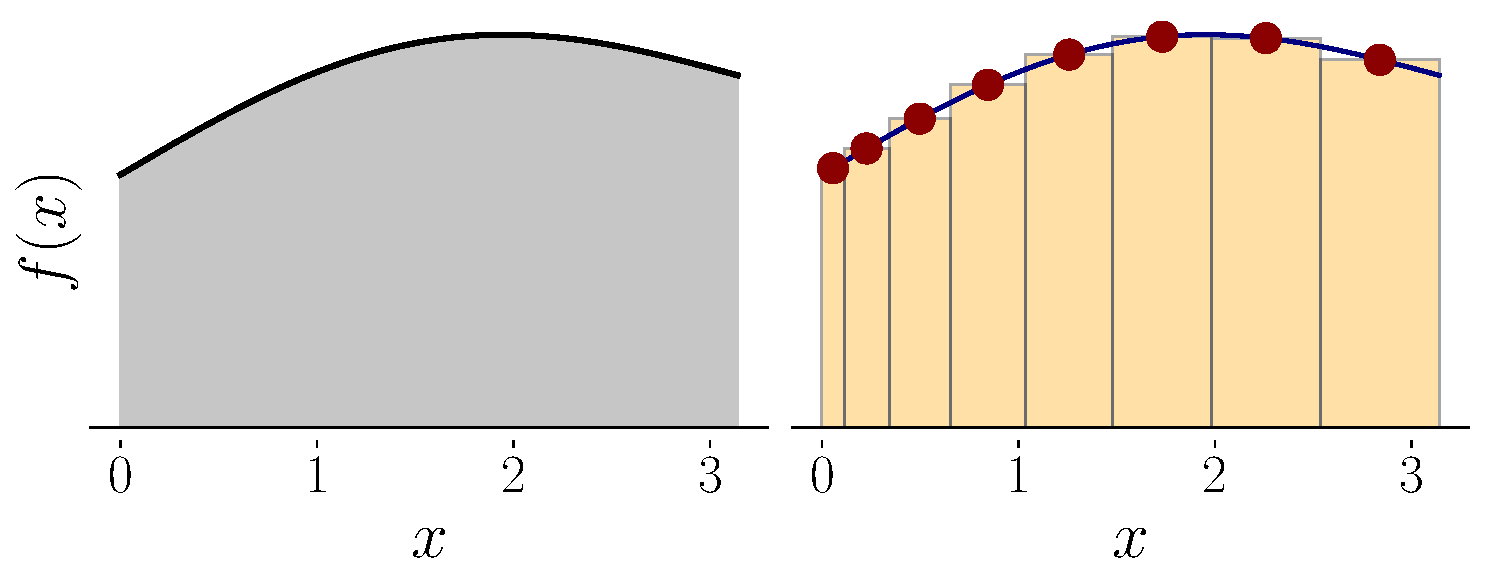
\includegraphics[width=\linewidth]{../plotting/figures/integral_illustration.pdf}
            \end{minipage}
        }

        \column{0.31\textwidth}
        \centering
        \setlength{\fboxsep}{5pt}
        \fcolorbox{mmdBlue!70!black}{mmdBlue!8}{%
            \begin{minipage}[t][0.40\textheight][t]{0.88\linewidth}
                \centering
                {\Large \mmdicon{mmdBlue!80!black}{$\sim$}}\\[0.08cm]
                {\bfseries Sampling / generative modelling}\\[0.12cm]
                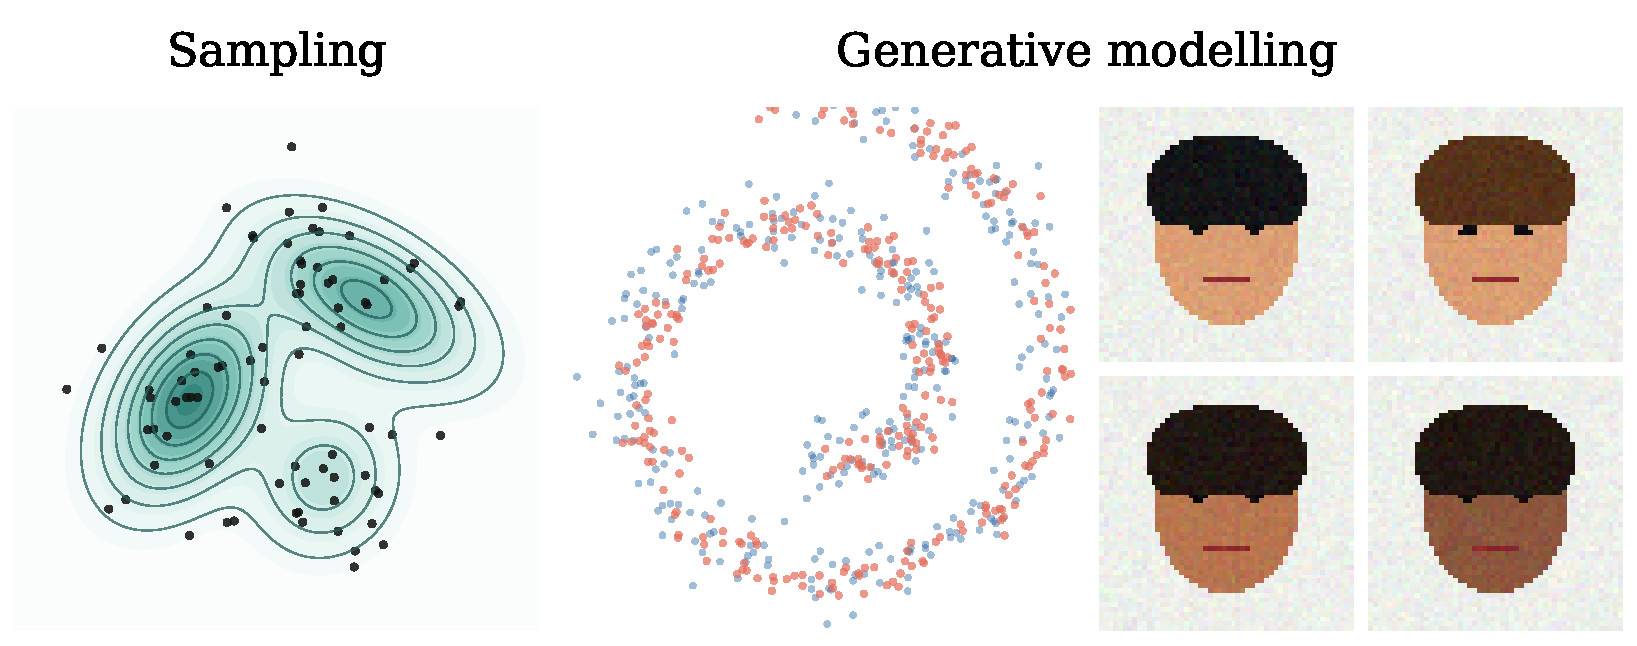
\includegraphics[width=\linewidth]{../plotting/figures/sampling_generative_illustration.pdf}
            \end{minipage}
        }

        \column{0.31\textwidth}
        \centering
        \setlength{\fboxsep}{5pt}
        \fcolorbox{mmdRed!70!black}{mmdRed!8}{%
            \begin{minipage}[t][0.40\textheight][t]{0.88\linewidth}
                \centering
                {\Large \mmdicon{mmdRed!80!black}{$\theta$}}\\[0.08cm]
                {\bfseries Statistical inference}\\[0.12cm]
                {\Large $\theta_{\mathrm{MMD}}$}\\[0.15cm]
                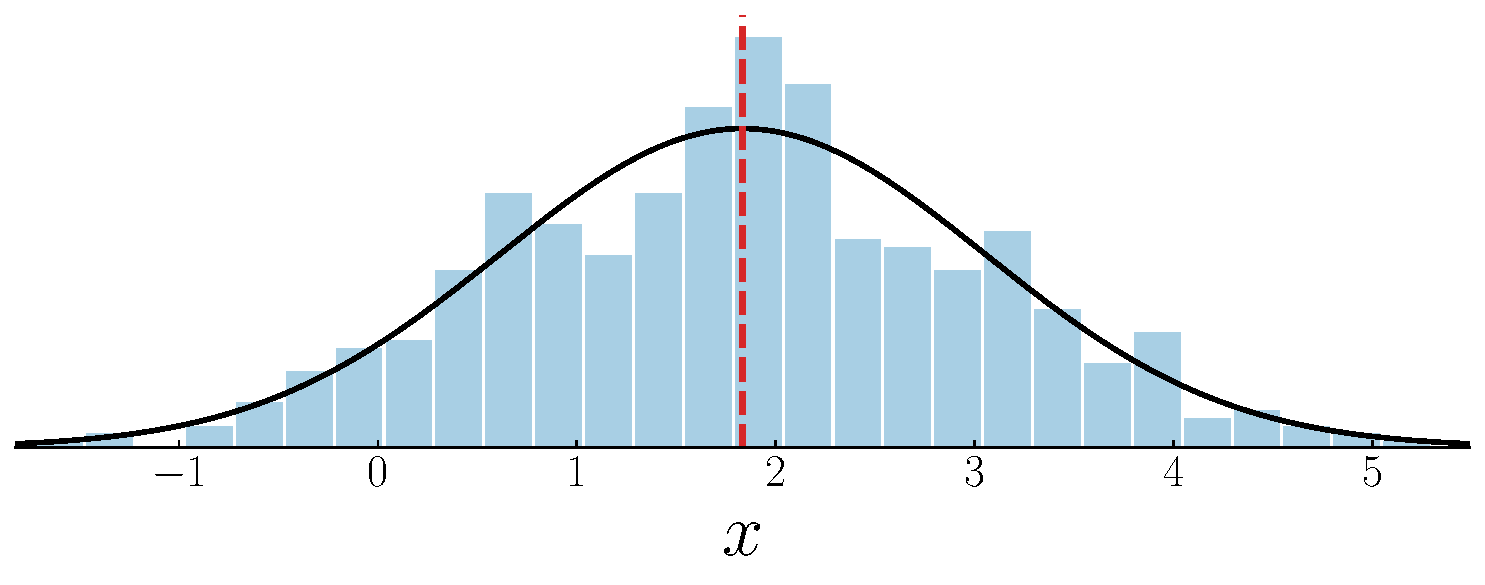
\includegraphics[width=\linewidth]{../plotting/figures/statistical_inference_illustration.pdf}
            \end{minipage}
        }
    \end{columns}
\end{frame}


\parttitleframe{Numerical Integration}

\begin{frame}{Part I: Numerical Integration}
    \centering
    {\large\bfseries Where do integrals appear in computer science?}\\[0.35cm]

    \begin{columns}[T,onlytextwidth]
        \column{0.31\textwidth}
        \centering
        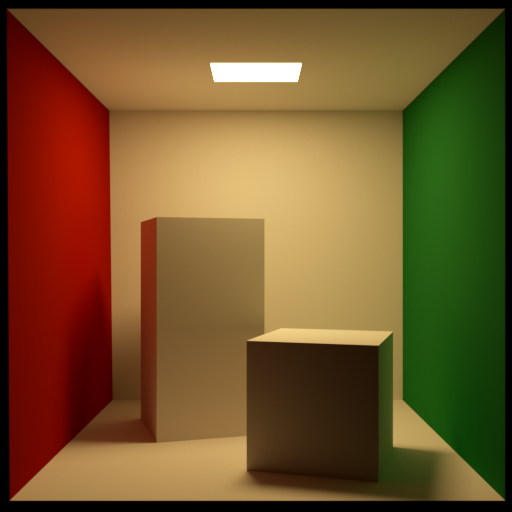
\includegraphics[height=0.48\textheight, width=\linewidth, keepaspectratio]{figures/web_apps/rendering.png}\\[0.12cm]
        {\bfseries Computer graphics}\\[-0.02cm]
        {\small Rendering}

        \column{0.31\textwidth}
        \centering
        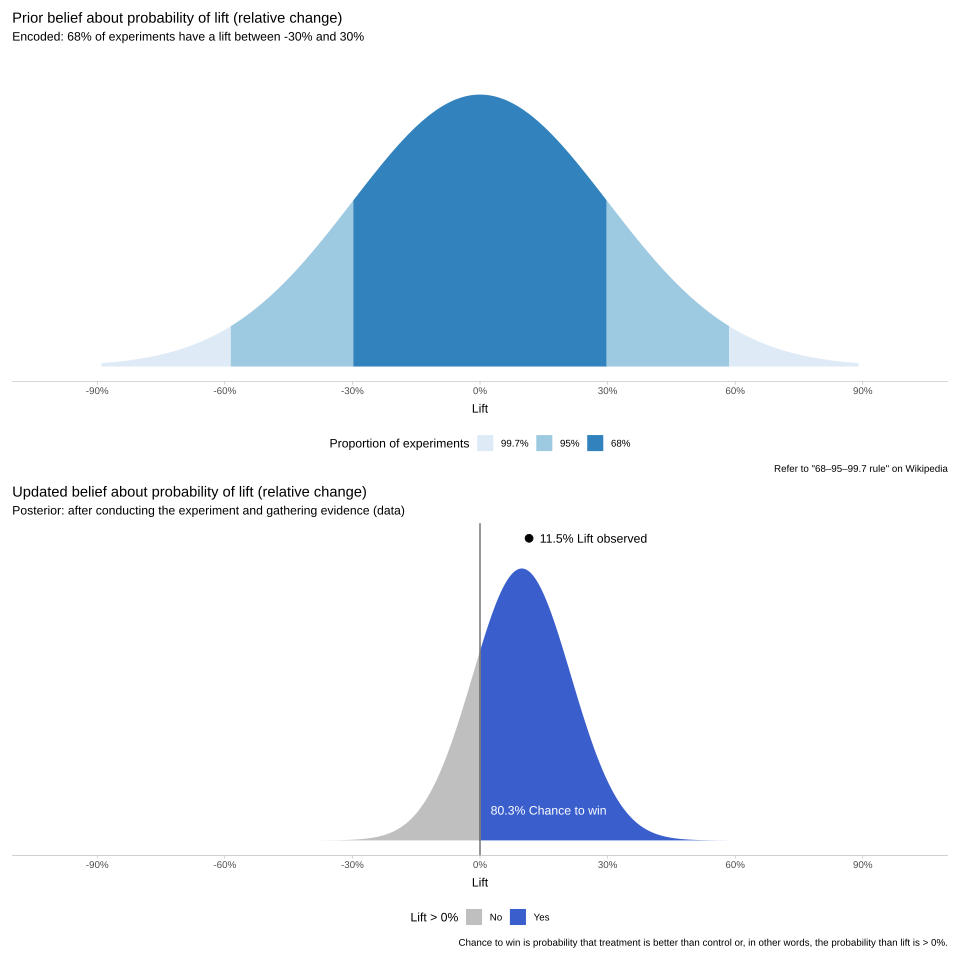
\includegraphics[height=0.48\textheight, width=\linewidth, keepaspectratio]{figures/web_apps/bayesian_ab.png}\\[0.12cm]
        {\bfseries Bayesian inference}\\[-0.02cm]
        {\small Posterior expectations}

        \column{0.31\textwidth}
        \centering
        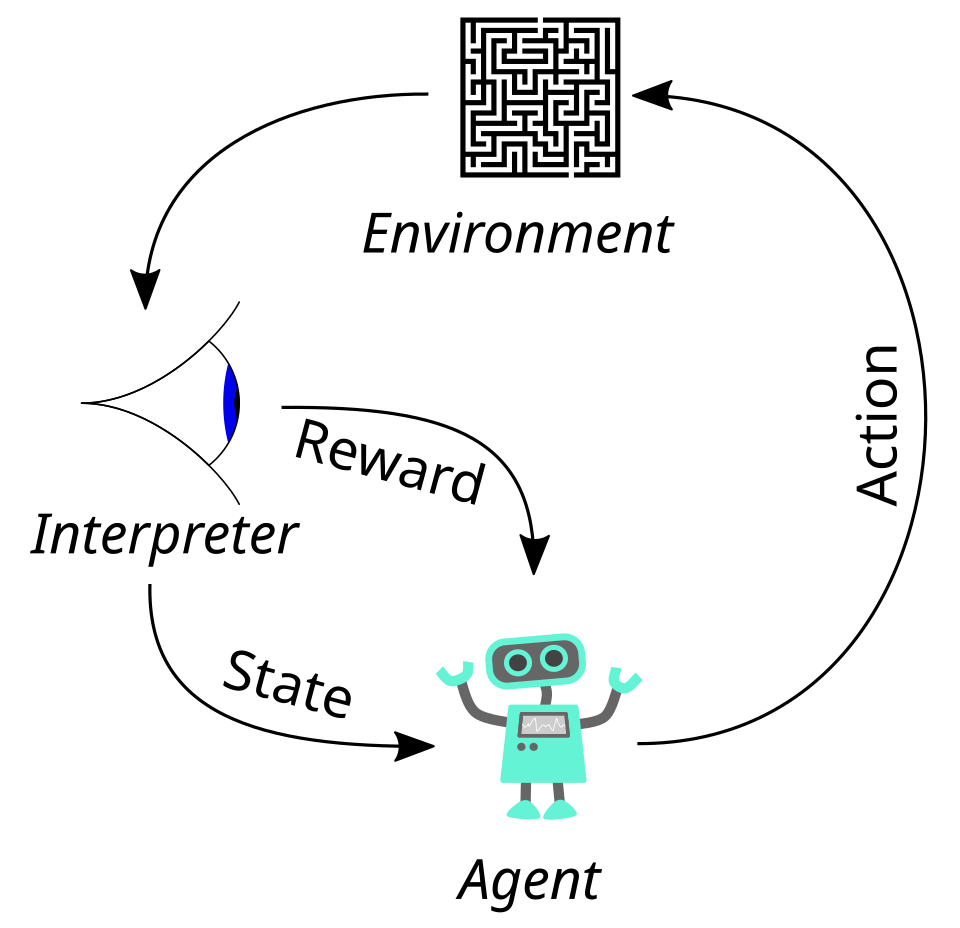
\includegraphics[height=0.48\textheight, width=\linewidth, keepaspectratio]{figures/web_apps/reinforcement_learning.png}\\[0.12cm]
        {\bfseries Reinforcement learning}\\[-0.02cm]
        {\small Expected returns}
    \end{columns}
\end{frame}

\begin{frame}{Part I: Numerical Integration}
    \begin{itemize}
        \item Given a function $f$ and a distribution $\Pb$, how to compute $\int f(x) \dd \Pb(x)$?
        \item Given a set of points $\{x_i\}_{i=1}^n$ and function evaluations $\{f(x_i)\}_{i=1}^n$.
        \item Quadrature rule:
        \begin{align*}
            \hat{I} = \sum_{i=1}^n w_i f(x_i).
        \end{align*}
        \item When $w_1=\cdots=w_n=1/n$, this is Monte Carlo. $\hat{I}_{MC} = \frac{1}{n}\sum_{i=1}^n f(x_i)$.
        \begin{align*}
            \E\left[|\hat{I}_{MC} - I|\right] = \mathcal{O}(n^{-1/2}).
        \end{align*}
        \item Or equivalently, to obtain an $\epsilon$-accurate estimate, we need $n = \mathcal{O}(\epsilon^{-2})$ samples.
    \end{itemize}
    \begin{exampleblock}{}
        \centering
        \textbf{Question:} Can we do better than $\mathcal{O}(n^{-1/2})$?
    \end{exampleblock}
    \begin{answerblock}{}
    \centering \textbf{Answer:} Find better weights $w_1,\ldots,w_n$.
    \end{answerblock}
\end{frame}

\begin{frame}{Part I: Numerical Integration}
    \begin{itemize}
        \item Suppose $f\in\calH$ is in the RKHS associated with $k$.
        \item Denote $\hat{\Pb}=\sum_{i=1}^n w_i \delta_{x_i}$ as the weighted empirical distribution.
        \begin{align*}
            \left|I - \hat{I} \right|^2 &= \left|\int f(x) \dd \Pb(x) - \sum_{i=1}^n w_i f(x_i)\right|^2
            \leq \|f\|_{\calH}^2 \cdot
            \mathrm{MMD}^2(\hat{\Pb}, \Pb) .         \end{align*}
        \item The right-hand side is the \red{worst-case} error of the quadrature rule. 
        \begin{align*}
            w_{1:n} &:= \arg\min_{w_{1:n}\in\R^n} \mmd\left(\sum_{i=1}^n w_i \delta_{x_i}, \Pb\right), \\ 
            w_{1:n} &= \E_{X \sim \Pb}[k(X, x_{1:n})]
            K(x_{1:n},x_{1:n})^{-1} . 
        \end{align*}
        \item The kernel quadrature (KQ) rule: $\hat{I}_{\mathrm{KQ}} = \sum_{i=1}^n w_i f(x_i)$.
    \end{itemize}
\end{frame}

\begin{frame}{Part I: Numerical Integration}
    \begin{answerblock}
        \centering \textbf{Rate:} KQ achieves \green{$\mathcal{O}(n^{-s/d})$} rate.
    \end{answerblock}
    \begin{itemize}
        \item \red{$s$} is the smoothness of $f$, $d$ is the dimension of input $x$. 
        \item Better than $\mathcal{O}(n^{-1/2})$ when $s > d/2$.
    \end{itemize}
    \centering
    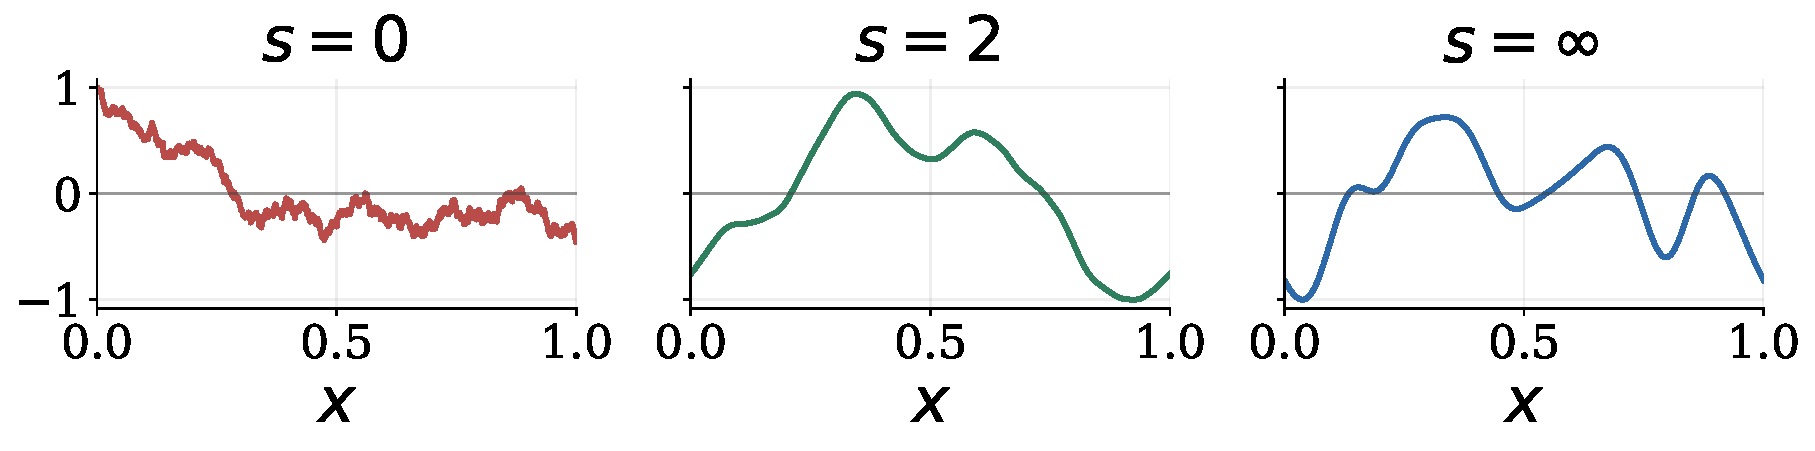
\includegraphics[width=0.96\linewidth]{../plotting/figures/kq_smoothness_illustration.pdf}
\end{frame}

\begin{frame}{Part I: Numerical Integration}
    \centering
    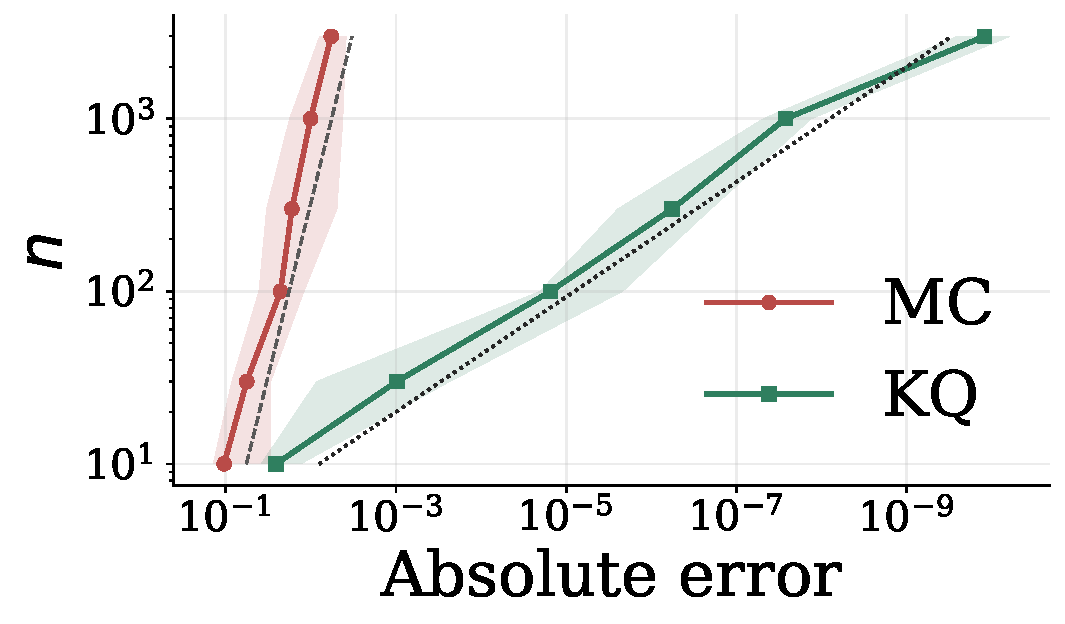
\includegraphics[width=0.62\linewidth]{../plotting/figures/kq_single_expectation_benchmark.pdf}
    \begin{itemize}
        \item $s=4$ and $d=1$. 
    \end{itemize}
\end{frame}

\begin{frame}{Part I: Numerical Integration}
    \centering
    \begin{itemize}
        \item Nested expectation: $\displaystyle
        I := \E_{\theta \sim \Qb}
        \left[
            f\left(\E_{X \sim \Pb_\theta}[g(X,\theta)]\right)
        \right]$
    \end{itemize}
        
    \vspace{0.15cm}
    \begin{tikzpicture}[
        scale=0.92,
        transform shape,
        outer/.style={circle, draw=mmdBlue!80!black, fill=mmdBlue!10, minimum size=6.5mm, font=\small},
        inner/.style={rounded corners=2pt, draw=mmdGreen!70!black, fill=mmdGreen!10, minimum width=2.35cm, minimum height=0.58cm, align=center, font=\small},
        evalbox/.style={rounded corners=2pt, draw=mmdRed!70!black, fill=mmdRed!8, minimum width=2.35cm, minimum height=0.58cm, align=center, font=\small},
        conn/.style={-{Latex[length=1.8mm]}, line width=0.7pt, mmdBlue!75!black},
        rowlabel/.style={font=\small\bfseries, text=mmdBlue!80!black, align=right, anchor=east}
    ]
        \node[rowlabel] at (-1.45,0.90) {outer samples};
        \node[outer] (th1) at (0,0.90) {$\theta_1$};
        \node[outer] (th2) at (2.50,0.90) {$\theta_2$};
        \node at (4.00,0.90) {$\cdots$};
        \node[outer] (thT) at (5.50,0.90) {$\theta_T$};

        \node[rowlabel] at (-1.45,-0.03) {inner samples};
        \node[inner] (x1) at (0,-0.03) {$x_{1:N}^{(1)} \sim \Pb_{\theta_1}$};
        \node[inner] (x2) at (2.50,-0.03) {$x_{1:N}^{(2)} \sim \Pb_{\theta_2}$};
        \node at (4.00,-0.03) {$\cdots$};
        \node[inner] (xT) at (5.50,-0.03) {$x_{1:N}^{(T)} \sim \Pb_{\theta_T}$};

        \node[rowlabel] at (-1.45,-0.84) {function evaluates};
        \node[evalbox] (g1) at (0,-0.84) {$g(x,\theta_1)$};
        \node[evalbox] (g2) at (2.50,-0.84) {$g(x,\theta_2)$};
        \node at (4.00,-0.84) {$\cdots$};
        \node[evalbox] (gT) at (5.50,-0.84) {$g(x,\theta_T)$};
        \node[font=\small\bfseries, text=mmdBlue!80!black] at (2.45,-1.54)
        {Total simulator evaluations: $N \times T$};
    \end{tikzpicture}

    \vspace{-0.15cm}
    \begin{columns}[T,onlytextwidth]
        \column{0.48\textwidth}
        \fcolorbox{mmdGreen!70!black}{mmdGreen!10}{%
        \begin{minipage}{0.94\linewidth}
            \vspace{0.10cm}
            {\centering\small\bfseries Stage I: inner KQ\par}\vspace{-0.25cm}
            \[
                \widehat{J}_{\mathrm{KQ}}(\theta_t)
                =
                \sum_{n=1}^{N}
                w^{\calX}_{n,t} g(x_n^{(t)},\theta_t)
            \]
            \vspace{-0.10cm}
        \end{minipage}}

        \column{0.48\textwidth}
        \fcolorbox{mmdBlue!80!black}{mmdBlue!10}{%
        \begin{minipage}{0.94\linewidth}
            \vspace{0.10cm}
            {\centering\small\bfseries Stage II: outer KQ\par}\vspace{-0.25cm}
            \[
                \widehat{I}_{\mathrm{NKQ}}
                =
                \sum_{t=1}^{T}
                w_t^{\Theta} f\left(\hat{J}^{\mathrm{KQ}}(\theta_t)\right)
            \]
            \vspace{-0.10cm}
        \end{minipage}}
    \end{columns}

    \vspace{0.15cm}
    \begin{tabular}{@{}c@{\hspace{0.24cm}}c@{}}
        {\bfseries Cost to achieve error $|I-\widehat{I}|\leq\Delta$:}
        &
        \resizebox{0.56\linewidth}{!}{%
        \begin{tabular}{@{}c@{\hspace{0.45cm}}c@{}}
            \toprule
            \textbf{NMC}: $\mathcal{O}(\Delta^{-4})$ or $\mathcal{O}(\Delta^{-3})$
            &
            \textbf{NQMC}: $\mathcal{O}(\Delta^{-2.5})$
            \\
            \textbf{MLMC}: $\mathcal{O}(\Delta^{-2})$
            &
            \textbf{NKQ}: $\tilde{\mathcal{O}}(\Delta^{-d_{\calX}/s_{\calX}-d_{\Theta}/s_{\Theta}})$
            \\
            \bottomrule
        \end{tabular}}
    \end{tabular}
\end{frame}

\begin{frame}{Part I: Numerical Integration}
    \centering
    \setlength{\fboxsep}{2pt}
    \fcolorbox{mmdGreen!70!black}{mmdGreen!6}{%
        \begin{minipage}[t][0.26\textheight][t]{0.95\linewidth}
            \centering
            {\bfseries Conditional Bayesian Quadrature~\textcolor{mmdGreen!80!black}{(UAI 2025)}}\\[-0.10cm]
            {\tiny\textcolor{graytext}{\underline{Z. Chen}, M. Naslidnyk, A. Gretton, F.-X. Briol}}\\[-0.10cm]

            \raggedright
            \begin{itemize}
                \setlength\itemsep{0pt}
                \item Extension to conditional expectations:
                $I(\theta)= \E_{X \sim p(\cdot \mid \theta)}[g(X,\theta)]$. 
                \item Weighted rule:
                $\hat{I}_{\mathrm{CBQ}}(\theta)
                := \sum_{t=1}^T \sum_{n=1}^N
                w_{n,t} g(x_n^{(t)},\theta_t)$.
            \end{itemize}
        \end{minipage}
    }

    \vspace{0.15cm}

    \fcolorbox{mmdBlue!70!black}{mmdBlue!6}{%
        \begin{minipage}[t][0.26\textheight][t]{0.95\linewidth}
            \centering
            {\bfseries Nested Expectations with Kernel Quadrature~\textcolor{mmdBlue!80!black}{(ICML 2025)}}\\[-0.10cm]
            {\tiny\textcolor{graytext}{\underline{Z. Chen}, M. Naslidnyk, F.-X. Briol}}\\[-0.10cm]

            \raggedright
            \begin{itemize}
                \setlength\itemsep{0pt}
                \item Extension to nested expectations: $I := \E_{\theta \sim \Qb}
\left[f\left(\E_{X \sim \Pb_\theta}[g(X,\theta)]\right)\right]$. 
                \item Weighted rule:
                $\hat{I}_{\mathrm{NKQ}}
                = \sum_{t=1}^T w_t^\Theta
                f\left(\sum_{n=1}^N
                w_{n,t}^{\calX}g(x_n^{(t)},\theta_t)\right)$.
            \end{itemize}
        \end{minipage}
    }

    \vspace{0.15cm}

    \fcolorbox{mmdGreen!70!black}{mmdGreen!6}{%
        \begin{minipage}[t][0.16\textheight][t]{0.95\linewidth}
            \centering
            {\bfseries BayesSum: Bayesian Quadrature in Discrete Spaces~\textcolor{mmdGreen!80!black}{(ProbNum 2026)}}\\[-0.10cm]
            {\tiny\textcolor{graytext}{S. S. Kang, F.-X. Briol, T. Karvonen, Z. Chen}}\\[-0.10cm]

            \raggedright
            \begin{itemize}
                \setlength\itemsep{0pt}
                \item Extension to sums: $I=\mathbb{E}_{X \sim \mathbb{P}}[f(X)]=\sum_{x \in \mathcal{X}} f(x) p(x)$. 
            \end{itemize}
        \end{minipage}
    }
\end{frame}

\begin{frame}[plain]
    \centering
    \vspace{0.20cm}
    {\Huge\bfseries Sampling / Generative Modelling}\\[0.28cm]

    \begin{tikzpicture}[
        x=1cm,
        y=1cm,
        panel/.style={rounded corners=2pt, line width=0.8pt},
        paneltitle/.style={font=\bfseries, text=mmdBlue!85!black},
        note/.style={font=\small, align=center, text=black},
        loc/.style={circle, fill=mmdRed!82!black, draw=white, line width=0.45pt, minimum size=4.2pt, inner sep=0pt},
        weightcircle/.style={circle, draw=none, fill=mmdGreen!55, opacity=0.32, inner sep=0pt},
        equalweight/.style={circle, draw=none, fill=mmdBlue!55, opacity=0.30, inner sep=0pt}
    ]
        \node[paneltitle] at (-3.50,1.52) {Quadrature};
        \node[note] at (-3.50,1.02) {fixed locations, choose weights};
        \draw[panel, draw=mmdGreen!65!black, fill=mmdGreen!3] (-5.55,-1.25) rectangle (-1.45,0.75);

        \foreach \x/\y/\r in {-4.72/-0.70/0.17,-4.18/0.10/0.34,-3.52/-0.42/0.58,-2.80/0.25/0.28,-2.18/-0.55/0.12} {
            \node[weightcircle, minimum size=\r cm] at ({\x+0.04},{\y-0.04}) {};
            \node[weightcircle, fill=mmdGreen!65, opacity=0.22, minimum size=\r cm] at (\x,\y) {};
            \node[loc] at (\x,\y) {};
        }

        \node[paneltitle] at (3.50,1.52) {Sampling / generation};
        \node[note] at (3.50,1.02) {equal weights, choose locations};
        \draw[panel, draw=mmdBlue!65!black, fill=mmdBlue!3] (1.45,-1.25) rectangle (5.55,0.75);

        \foreach \x/\y in {2.08/-0.72,2.72/-0.12,3.28/-0.58,3.88/0.18,4.70/-0.42} {
            \node[equalweight, minimum size=0.34cm] at ({\x+0.04},{\y-0.04}) {};
            \node[equalweight, fill=mmdBlue!70, opacity=0.18, minimum size=0.34cm] at (\x,\y) {};
            \node[loc] at (\x,\y) {};
        }
    \end{tikzpicture}
\end{frame}

\begin{frame}{Part II: Sampling / Generative modelling}
    \centering 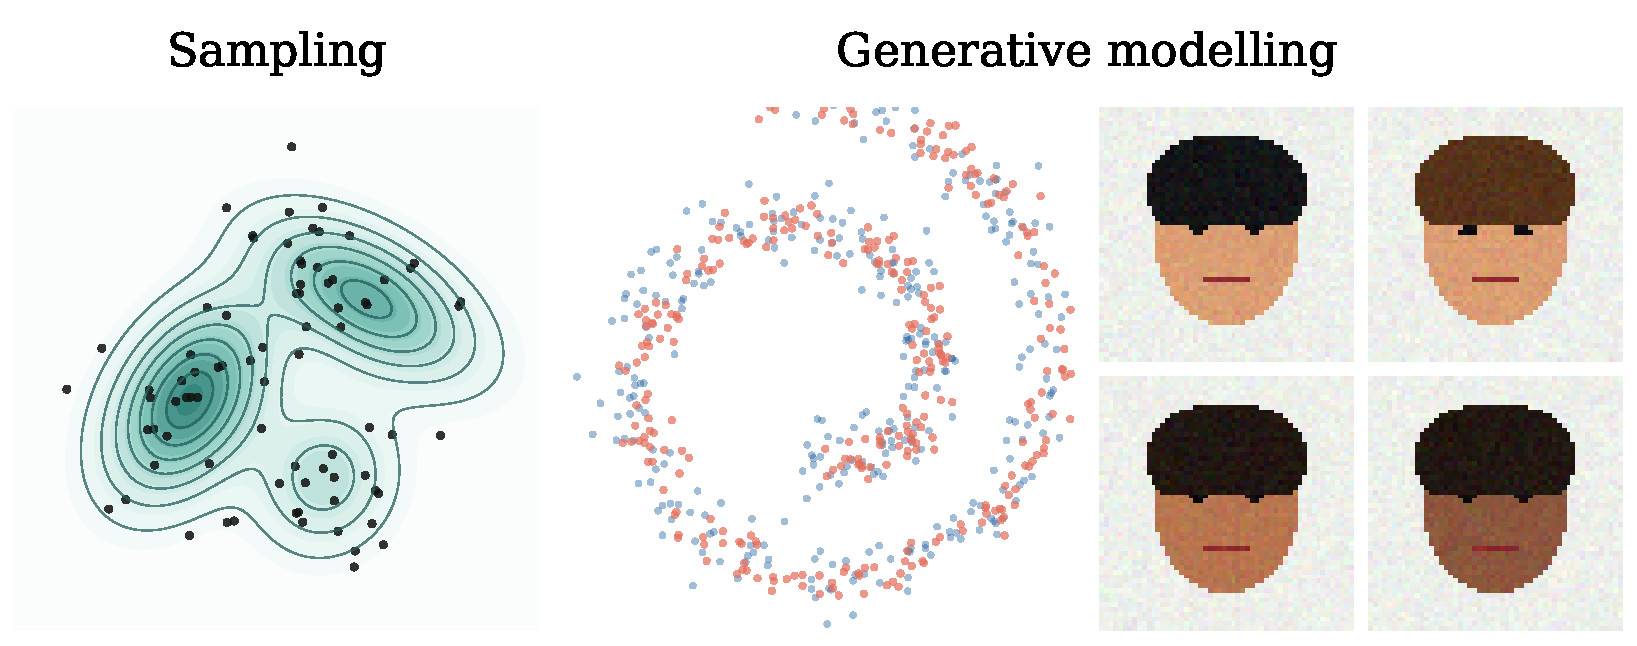
\includegraphics[width=0.70\linewidth]{../plotting/figures/sampling_generative_illustration.pdf}\\[0.12cm]
    \begin{itemize}
        \item Given a target distribution $\Qb$, how to draw samples $\{x_i\}_{i=1}^n$ from it?
        \begin{itemize}
            \item When $\Qb$ is known up to normalization, this is sampling.
            \item When $\Qb$ is known with i.i.d samples, this is generative modelling.
        \end{itemize}
    \end{itemize}
\end{frame}

\begin{frame}{Part II: Sampling / Generative modelling}
    \begin{exampleblock}{}
    \centering
        \textbf{Problem}: How to learn a target probability distribution $\Qb$ on $\R^d$.
    \end{exampleblock}
    \begin{itemize}
        \item This problem can be written as an \blue{optimization} problem on $\calP(\R^d)$, the space of probability distributions.
        \begin{align*}
            \arg\min_{\Pb \in \calP(\R^d)} D(\Pb, \Qb) . 
        \end{align*}
        \item Here $D$ is a similarity metric or distance, e.g. Kullback–Leibler divergence / MMD. 
        \begin{itemize}
            \item $D(\Pb_1 , \Pb_2) = 0$ if and only if $\Pb_1=\Pb_2$. 
        \end{itemize}
        \item How to find the minimum? Gradient descent!
    \end{itemize}
\end{frame}


\begin{frame}{Part II: Sampling / Generative modelling}
    \begin{exampleblock}{}
    \centering
        \textbf{Question}: Wait... How to define gradients on $\calP(\R^d)$?
    \end{exampleblock}
    \begin{answerblock}
        \centering \textbf{Answer}: Wassserstein gradient !~\citep{otto2001geometry}
    \end{answerblock}
    \vspace{0.25cm}
    \centering 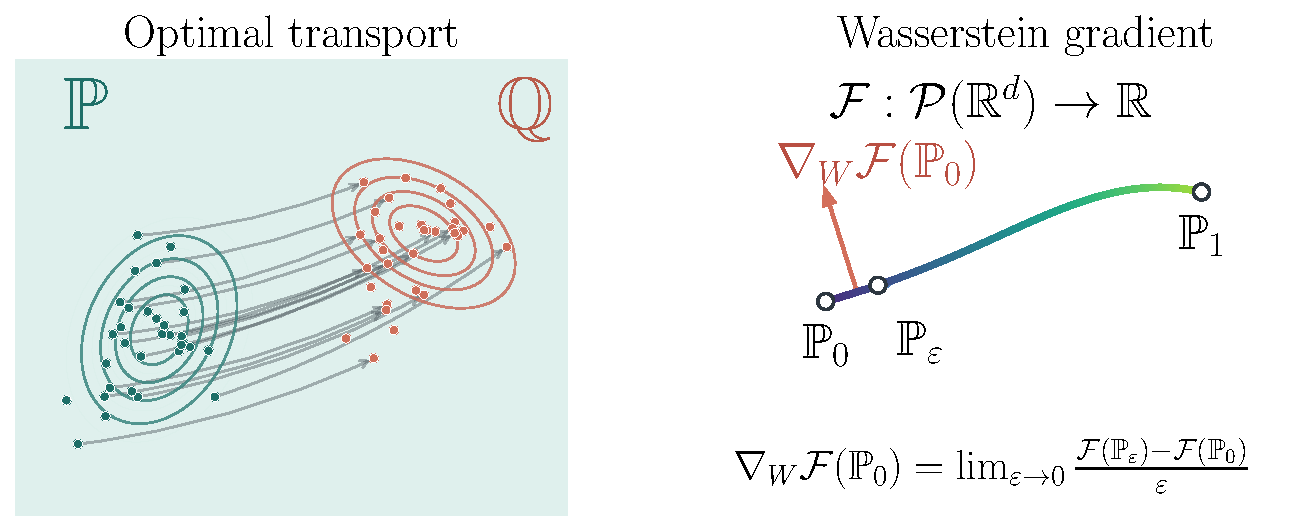
\includegraphics[width=0.80\linewidth]{../plotting/figures/ot_wasserstein_gradient_illustration.pdf}\\[0.12cm]
\end{frame}

\begin{frame}{Part II: Sampling / Generative modelling}
    \begin{itemize}
        \item Unsurprisingly, we use MMD as the divergence.
    \begin{talign*}
        \arg\min_{\Pb \in \calP(\R^d)} \mmd^2(\Pb, \Qb) . 
    \end{talign*}
        \item A (Wasserstein) gradient descent of $\mmd^2(\Pb, \Qb)$ gives a sequence of distributions: $\Pb_0, \Pb_1, \ldots, \Pb_t$~\citep{arbel2019maximum}.
        \begin{itemize}
            \item In the limit, $\Pb_t$ converges to $\Qb$ and $\mmd(\Pb_t, \Qb) \to 0$ (or not?). 
        \end{itemize}
    \end{itemize}
    \vspace{0.25cm}
    \centering 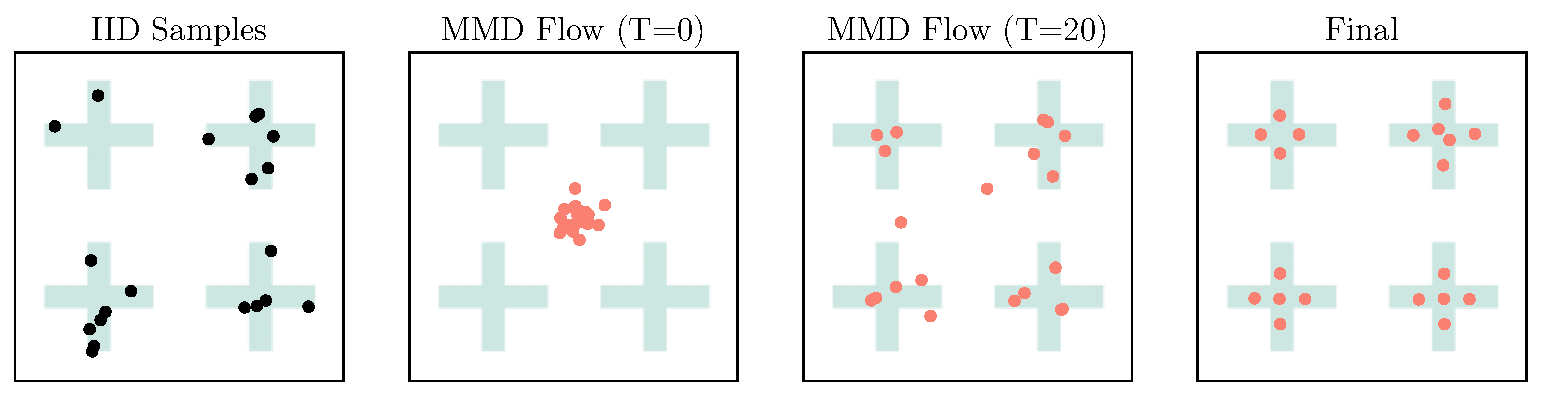
\includegraphics[width=0.85\linewidth]{../plotting/figures/illustration_sampling.pdf}\\[0.12cm]
    \begin{itemize}
        \item MMD flow generates more \red{uniform} samples.
    \end{itemize}
\end{frame}

\begin{frame}{Part II: Sampling / Generative modelling}
    \centering 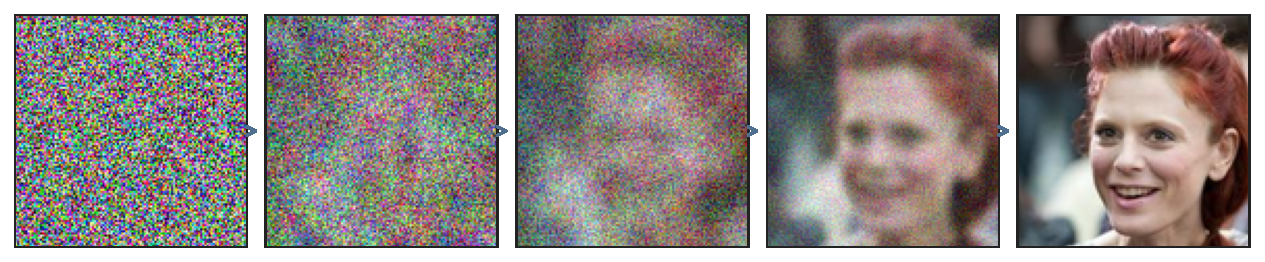
\includegraphics[width=0.80\linewidth]{../plotting/figures/generative_reverse_noising_celeba.pdf}\\[0.12cm]

    \begin{itemize}
        \item MMD flow does not outperform diffusion-based generative models~\citep{galashov2024deep}.
        \item A novel framework of generative modelling \& sampling.
    \end{itemize}
\end{frame}

\begin{frame}{Part II: Sampling / Generative modelling}
    \begin{exampleblock}{}
        \centering \textbf{Challenge:}  Non-convexity of the squared MMD objective: $\lim_{t\to\infty}\mmd^2(\Pb_t, \Qb) > 0$. 
    \end{exampleblock}
    \begin{itemize}
        \item $\chi^2(\mu\|\pi)$ is convex in $\mu$~\citep{ohta2011displacement}, yet hard to implement.  
        \item DrMMD \blue{interpolates} between MMD ($\lambda=\infty$) and $\chi^2$ ($\lambda=0$).
    \end{itemize}
    \begin{align*}
        \operatorname{DrMMD}(\mu, \pi)=\sup_{f \in \mathcal{H}:\|f\|_{L_2(\mu)}^2+\lambda\|f\|_{\mathcal{H}}^2 \leq 1} \int f \mathrm{~d}(\mu-\pi) .
    \end{align*}
    \vspace{-0.15cm}
    \begin{itemize}
        \item DrMMD flow converges in KL divergence: $\lim_{t\to\infty}\mathrm{KL}(\Pb_t, \Qb)=0$.
        \begin{itemize}
            \item When $\pi$ is `Gaussian-like'. 
        \end{itemize}
    \end{itemize}
\end{frame}


\begin{frame}{Part II: Sampling / Generative modelling}
    \centering
    \setlength{\fboxsep}{2pt}
    \fcolorbox{mmdBlue!70!black}{mmdBlue!6}{%
        \begin{minipage}[t][0.23\textheight][t]{0.95\linewidth}
            \centering
            {\bfseries (De)-regularized MMD Gradient Flow~\textcolor{mmdBlue!80!black}{(JMLR 2025)}}\\[-0.10cm]
            {\tiny\textcolor{graytext}{\underline{Z. Chen}, A. Mustafi, P. Glaser, A. Korba, A. Gretton, B. K. Sriperumbudur}}\\[-0.10cm]

            \raggedright
            \begin{itemize}
                \item DrMMD interpolates between MMD and $\chi^2$ divergence.
                \item Convergence in KL divergence: $\lim_{t\to\infty}\mathrm{KL}(\Pb_t, \Qb)=0$. 
            \end{itemize}
        \end{minipage}
    }

    \vspace{0.20cm}

    \fcolorbox{mmdGreen!70!black}{mmdGreen!6}{%
        \begin{minipage}[t][0.50\textheight][t]{0.95\linewidth}
            \centering
            {\bfseries Sobolev Regularized MMD Gradient Flow~\textcolor{mmdGreen!80!black}{(Arxiv)}}\\[-0.10cm]
            {\tiny\textcolor{graytext}{C. Tian, B. K. Sriperumbudur, A. Gretton, \underline{Z. Chen}}}\\[-0.10cm]

            \raggedright
            \begin{itemize}
                \item Gradient regularization on the critic~\citep{mroueh2019sobolev}.
                \begin{align*}
                    \operatorname{SrMMD}(\mu, \pi)=\sup _{f \in \mathcal{H}:\|\nabla f\|_{L_2^d(\mu)}^2+\lambda\|f\|_{\mathcal{H}}^2 \leq 1} \int f \mathrm{~d}(\mu-\pi) .
                \end{align*}
                \item Convergence in MMD: $\lim_{t\to\infty}\mathrm{MMD}(\Pb_t, \Qb)=0$.
                \item No conditions on $\pi$. 
            \end{itemize}
        \end{minipage}
    }
\end{frame}

\begin{frame}{Part II: Sampling / Generative modelling}
    \begin{exampleblock}{}
        \centering \textbf{Empirical observation:} \\
        (Wasserstein) gradient flows give samples more \red{uniform} than i.i.d samples~\citep{xu2022accurate}.
    \end{exampleblock}
    \centering 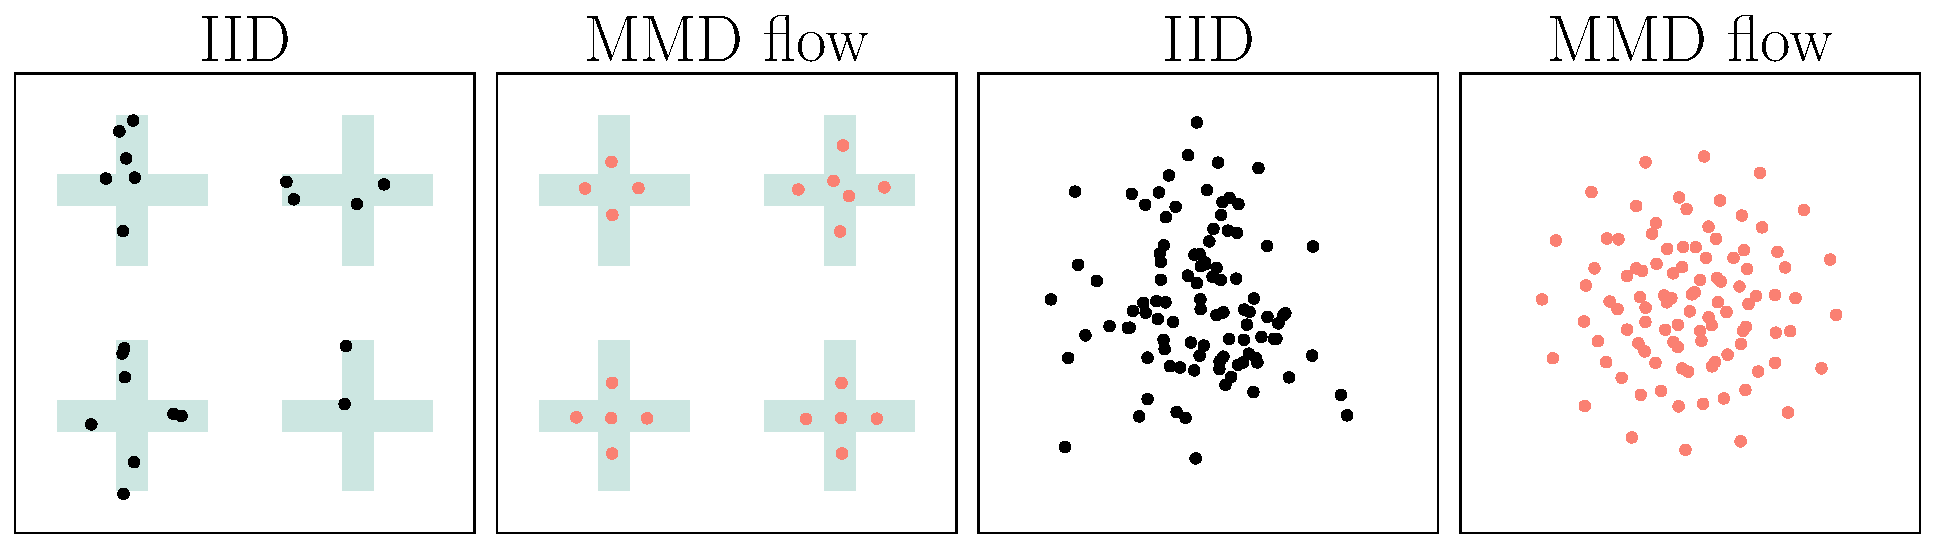
\includegraphics[width=0.75\linewidth]{../plotting/figures/sampling_four_panel_summary.pdf}\\[0.12cm]
    \begin{itemize}
        \item However, theoretical rate can hardly beat Monte Carlo: $n^{-1/2}$.
    \end{itemize}
\end{frame}


\begin{frame}{Part II: Sampling / Generative modelling}
    \begin{itemize}
        \item For any $i\in\{1, \ldots, n\}$:  
    \begin{align*}
        \nabla_{x_i} \operatorname{MMD}^2\left(\mu, \frac{1}{n} \sum_{j=1}^n \delta_{x_j}\right)=0 
        \Longrightarrow \frac{1}{n} \sum_{j=1}^n \nabla_1 k\left(x_i, x_j\right)-\int \nabla_1 k\left(x_i, y\right) \mathrm{d} \mu(y)=0. 
    \end{align*}
        \item Exact integration on $x \mapsto \nabla_1 k\left(x_i, x\right)$.
    \end{itemize}
    \begin{exampleblock}{}
        \centering \textbf{Exact integration subspace:} 
        \vspace{-0.20cm}
        \begin{align*}
        \mathcal{G}_n := \operatorname{span}\Bigl\{
        \nabla_1 k(x_i,\cdot) : i\in\{1, \ldots, n\}. \Bigr\} \subset \mathcal{H}.
        \end{align*}
    \end{exampleblock}
    \begin{itemize}
        \item As $n\to\infty$, $\mathcal{G}_n$ approximates the whole RKHS $\calH$ up to constant functions.
        \item Stationary MMD points achieve \blue{$o(n^{-1/2})$} rate for numerical integration. 
    \end{itemize}
\end{frame}


\begin{frame}{Part II: Sampling / Generative modelling}
    \centering
    \setlength{\fboxsep}{2pt}
    \fcolorbox{mmdRed!70!black}{mmdRed!6}{%
        \begin{minipage}[t][0.25\textheight][t]{0.95\linewidth}
            \centering
            {\bfseries Stationary MMD Points~\textcolor{mmdRed!80!black}{(ICML 2026)}}\\[-0.10cm]
            {\tiny\textcolor{graytext}{\underline{Z. Chen}, T. Karvonen, H. Kanagawa, F.-X. Briol, C. J. Oates}}\\[-0.10cm]

            \raggedright
            \begin{itemize}
                \item Samples from MMD flow are better for numerical integration than IID samples. 
                \item IID samples: $\mathcal{O}(n^{-1/2})$, stationary MMD points: $o(n^{-1/2})$.
            \end{itemize}
        \end{minipage}
    }

    \vspace{0.20cm}

    \fcolorbox{orange!80!black}{orange!7}{%
        \begin{minipage}[t][0.32\textheight][t]{0.95\linewidth}
            \centering
            {\bfseries Thinned Mean Field Langevin Dynamics~\textcolor{orange!80!black}{(ICML 2026)}}\\[-0.10cm]
            {\tiny\textcolor{graytext}{\underline{Z. Chen}, H. Kanagawa, F.-X. Briol, C. J. Oates, L. Mackey}}\\[-0.10cm]

            \raggedright
            \begin{itemize}
                \item Computational cost of MMD flow is $\calO(n^2)$ due to pair-wise interaction.
                \item Reduce cost to $\mathcal{O}(n^{1.5})$ without sacrificing the sample quality.
                \item Kernel thinning! 
            \end{itemize}
        \end{minipage}
    }
\end{frame}

\begin{frame}[plain]
    \centering
    \vspace{0.10cm}
    {\Huge\bfseries Statistical Inference}\\[0.28cm]

    \begin{columns}[T,onlytextwidth]
        \column{0.48\textwidth}
        \fcolorbox{mmdBlue!75!black}{mmdBlue!7}{%
        \begin{minipage}[t][0.3\textheight][t]{0.94\linewidth}
            \vspace{0.50cm}
            \centering
            {\Large\bfseries MMD flow}\\[-0.40cm]
            \[
                \arg\min_{\Pb \in \calP(\R^d)}
                \mathrm{MMD}^2(\Pb,\Qb)
            \]
        \end{minipage}}

        \column{0.48\textwidth}
        \fcolorbox{mmdGreen!70!black}{mmdGreen!7}{%
        \begin{minipage}[t][0.3\textheight][t]{0.94\linewidth}
            \vspace{0.50cm}
            \centering
            {\Large \bfseries Minimum MMD inference}\\[-0.40cm]
            \[
                \theta_{\mathrm{MMD}}
                =
                \arg\min_{\theta \in \Theta}
                \mathrm{MMD}^2(\Pb_\theta,\Qb)
            \]
        \end{minipage}}
    \end{columns}
\end{frame}

\begin{frame}{Part III: Statistical inference}
    \centering
    {\large\bfseries Where does statistical inference appear in computer science?}\\[0.35cm]

    \begin{columns}[T,onlytextwidth]
        \column{0.31\textwidth}
        \centering
        \fcolorbox{mmdBlue!70!black}{mmdBlue!8}{%
            \begin{minipage}[c][0.46\textheight][c]{0.84\linewidth}
                \centering
                \begin{tikzpicture}[scale=0.62, every node/.style={font=\scriptsize}]
                    \node[
                        rounded corners=3pt,
                        fill=mmdBlue!18,
                        draw=mmdBlue!80!black,
                        thick,
                        minimum width=0.95cm,
                        minimum height=0.56cm
                    ] (theta) at (-1.25,0.72) {$\theta$};
                    \node[
                        rounded corners=3pt,
                        fill=mmdGreen!16,
                        draw=mmdGreen!80!black,
                        thick,
                        minimum width=1.38cm,
                        minimum height=0.56cm
                    ] (sim) at (0,0.08) {simulator};
                    \node[
                        rounded corners=3pt,
                        fill=mmdRed!16,
                        draw=mmdRed!80!black,
                        thick,
                        minimum width=0.95cm,
                        minimum height=0.56cm
                    ] (x) at (1.25,-0.56) {$x$};
                    \draw[-{Latex[length=2mm]}, thick, dashed]
                        (x.south) .. controls (1.05,-1.32) and (-1.3,-1.28) ..
                        node[pos=0.52, below] {$p(\theta|x)$} (theta.south west);
                \end{tikzpicture}\\[0.14cm]
                {\bfseries Simulation-based\\inference}\\[-0.10cm]
                {\small Infer parameters from simulator outputs.}
            \end{minipage}
        }

        \column{0.31\textwidth}
        \centering
        \fcolorbox{mmdRed!70!black}{mmdRed!8}{%
            \begin{minipage}[c][0.46\textheight][c]{0.84\linewidth}
                \centering
                \begin{tikzpicture}[scale=0.72, every node/.style={font=\scriptsize}]
                    \draw[very thick, mmdBlue!80!black] (-1.45,-0.75) -- (-1.45,1.1) -- (-0.15,1.1);
                    \draw[very thick, mmdRed!80!black] (0.15,-0.75) -- (1.45,-0.75) -- (1.45,1.1);
                    \node[font=\footnotesize\bfseries, mmdBlue!80!black] at (-0.75,0.35) {$H_0$};
                    \node[font=\footnotesize\bfseries, mmdRed!80!black] at (0.75,0.35) {$H_1$};
                    \draw[-{Latex[length=2mm]}, thick] (-1.65,-0.95) -- (1.65,-0.95) node[right] {data};
                    \draw[dashed, thick] (0,-1.02) -- (0,1.28);
                \end{tikzpicture}\\[0.15cm]
                {\bfseries Hypothesis testing}\\[-0.02cm]
                {\small Is the data compatible with a class of models?}
            \end{minipage}
        }

        \column{0.31\textwidth}
        \centering
        \fcolorbox{mmdGreen!65!black}{mmdGreen!8}{%
            \begin{minipage}[c][0.46\textheight][c]{0.84\linewidth}
                \centering
                \begin{tikzpicture}[scale=0.72, every node/.style={font=\scriptsize}]
                    \draw[-{Latex[length=2mm]}, thick] (-1.65,-1.0) -- (1.65,-1.0) node[right] {$x$};
                    \draw[-{Latex[length=2mm]}, thick] (-1.65,-1.0) -- (-1.65,1.25) node[above] {$y$};
                    \fill[mmdGreen!18] plot[smooth, samples=80, domain=-1.35:1.35]
                        (\x,{0.55*sin(1.5*\x r)+0.45})
                        -- plot[smooth, samples=80, domain=1.35:-1.35]
                        (\x,{0.55*sin(1.5*\x r)-0.45}) -- cycle;
                    \draw[very thick, mmdGreen!80!black] plot[smooth, samples=80, domain=-1.35:1.35]
                        (\x,{0.55*sin(1.5*\x r)});
                    \foreach \x/\y in {-1.2/-0.6,-0.55/-0.35,0.15/0.1,0.85/0.62,1.25/0.48} {
                        \fill[mmdBlue!80!black] (\x,\y) circle (2.4pt);
                    }
                \end{tikzpicture}\\[0.15cm]
                {\bfseries Uncertainty}\\[-0.02cm]
                {\small How confident should a prediction be?}
            \end{minipage}
        }
    \end{columns}
\end{frame}

\begin{frame}{Part III: Statistical inference}
    \begin{itemize}
        \item Given a parametric model $\{\Pb_\theta\}_{\theta\in\Theta\subseteq\R^p}$. 
        \item Infer the parameter $\theta$ that best explains an unknown data distribution $\Qb$.
        \item Maximum likelihood estimation is the most popular:
        \begin{align*}
            \theta_{\mathrm{MLE}} = \arg\max_{\theta\in\Theta} \E_{X\sim\Qb}[\log p_\theta(X)]. 
        \end{align*}
    \end{itemize}
\end{frame}

\begin{frame}{Part III: Statistical inference}
    \centering
    {\large\bfseries What is not captured by maximum likelihood?}\\[0.2cm]

    \begin{columns}[T,onlytextwidth]
        \column{0.48\textwidth}
        \begin{block}{Likelihood-free simulators}
            When $\Pb_\theta$ is a scientific simulator: we can sample $x\sim p_\theta(x)$,
            but cannot evaluate the density $p_\theta(x)$.

            \par\vspace{0.18cm}
            \centering
            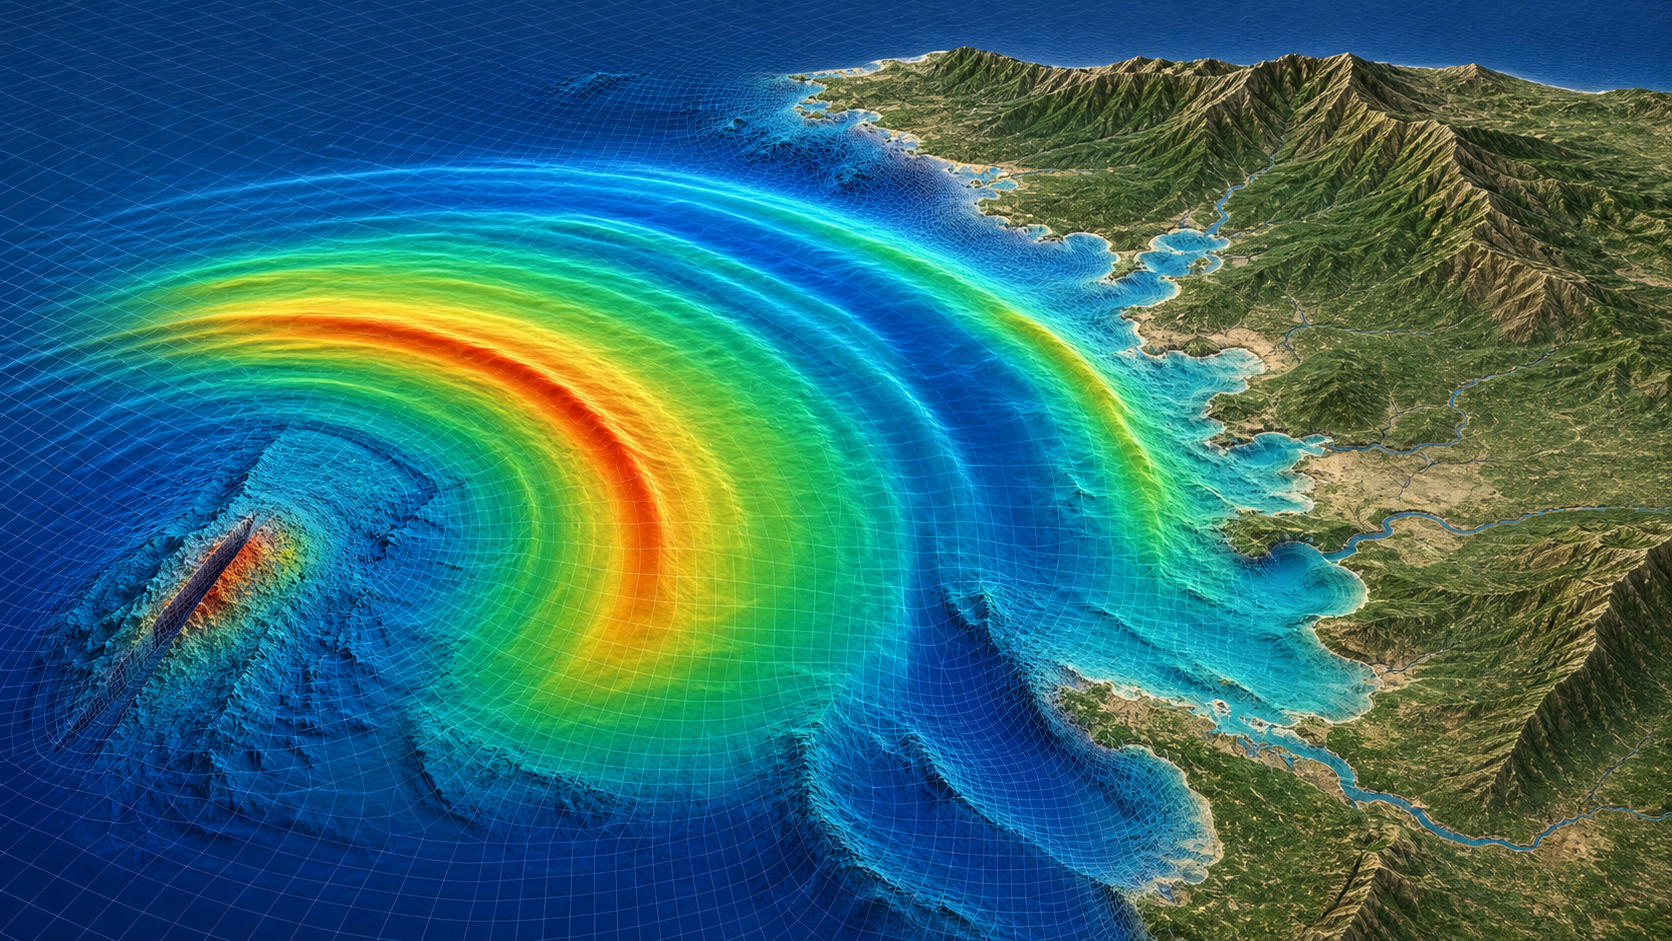
\includegraphics[width=0.92\linewidth,trim=0 170bp 0 170bp,clip]{figures/tsunami_simulator.png}
        \end{block}

        \column{0.48\textwidth}
        \begin{block}{Robustness}
            A few contaminated observations can strongly move the fitted parameter.
            
            \par\vspace{0.30cm}
            \centering
            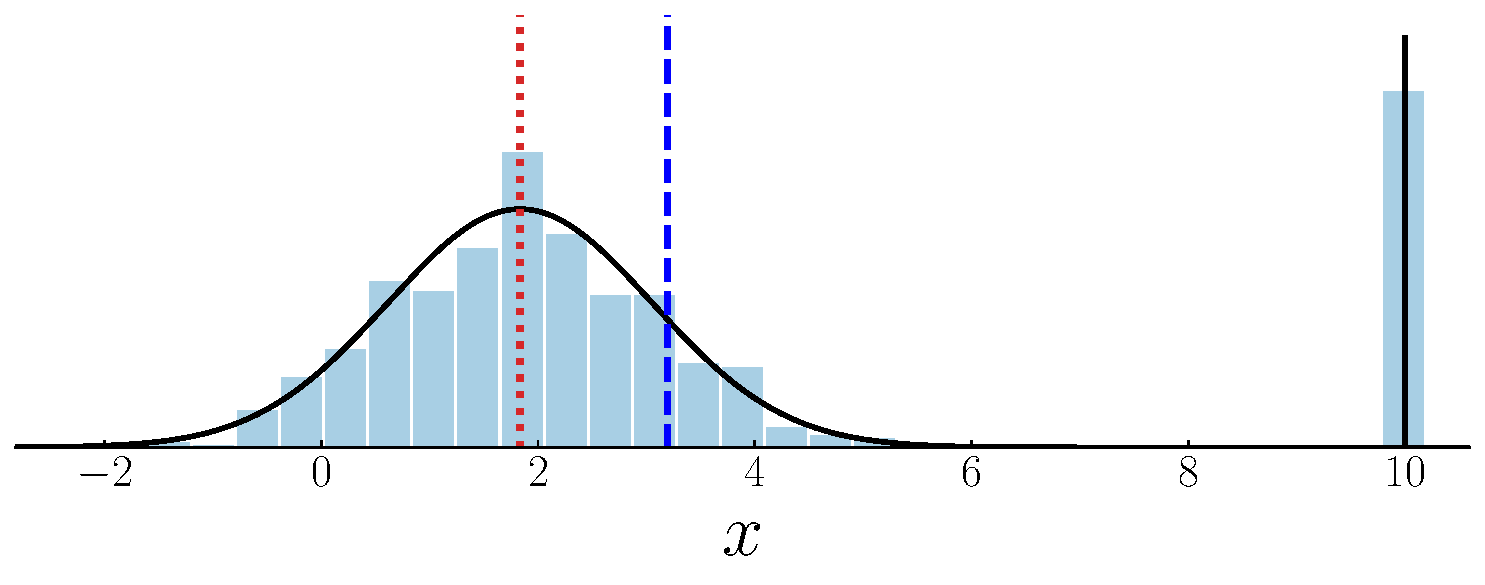
\includegraphics[width=0.95\linewidth]{../plotting/figures/statistical_inference_outlier_illustration.pdf}
        \end{block}
    \end{columns}
\end{frame}

\begin{frame}{Part III: Statistical inference}
    \begin{itemize}
        \item Minimum MMD estimator~\citep{briol2019statistical,cherief2022finite}
        \begin{align*}
            \theta_{\mathrm{MMD}}
            &= \arg\min_{\theta\in\Theta} \mathrm{MMD}^2(\Pb_\theta, \Qb) \\
            &= \arg\min_{\theta\in\Theta}
            \Big\{
            \E_{x,x'\sim\Pb_\theta}[k(x,x')]
            -2\E_{x\sim\Pb_\theta, y\sim\Qb}[k(x,y)]
            + \mathrm{const}
            \Big\}.
        \end{align*}

    \end{itemize}

    \vspace{0.10cm}
    \begin{columns}[T,onlytextwidth]
        \column{0.48\textwidth}
        \begin{exampleblock}{}
            \centering \textbf{Challenge 1:} Likelihood-free inference?
        \end{exampleblock}
        
        \begin{answerblock}
            \centering {\Large\checkmark} Only requires samples from $\Pb_\theta$ and $\Qb$.\\
        \end{answerblock}

        \column{0.48\textwidth}
        \begin{exampleblock}{}
            \centering \textbf{Challenge 2:} Robustness to outliers?
        \end{exampleblock}
        \begin{answerblock}
            \centering {\Large\checkmark} Bounded effects under bounded kernels. \\
        \end{answerblock}
    \end{columns}
\end{frame}

\begin{frame}{Part III: Statistical inference}
    \begin{exampleblock}{}
        \centering \textbf{Question:} How to reliably find $\theta_{\mathrm{MMD}}$?
    \end{exampleblock}
    \begin{columns}[T,onlytextwidth]
        \column{0.66\textwidth}
        \begin{itemize}
            \setlength\itemsep{0.12cm}
            \item MMD flow:
            \[
                \Pb_{t+1}
                =
                (\Id - \gamma \nabla f_{\Pb_t,\Qb})_{\#}\Pb_t .
            \]
            \item MMD flow converges globally.
            \begin{itemize}
                \item Adaptive lengthscale, DrMMD, SrMMD, etc.
            \end{itemize}
            \item Consider $\Pb_\theta=(T_\theta)_{\#}\rho$:
            \[
                \Pb_{\theta_{t+1}} = (T_{\theta_t - \gamma \Delta \theta_t})_\# \rho .
            \]
            \item Choose $\Pb_{\theta_{t+1}}$ closest to the MMD flow iterate $\Pb_{t+1}$.
            \item $\lim_{t\to\infty} \mmd(\Pb_{\theta_t}, \Qb) = \min_{\theta} \mmd(\Pb_{\theta}, \Qb)$. 
        \end{itemize}

        \column{0.33\textwidth}
        \begin{minipage}[c][0.64\textheight][c]{\linewidth}
            \centering
            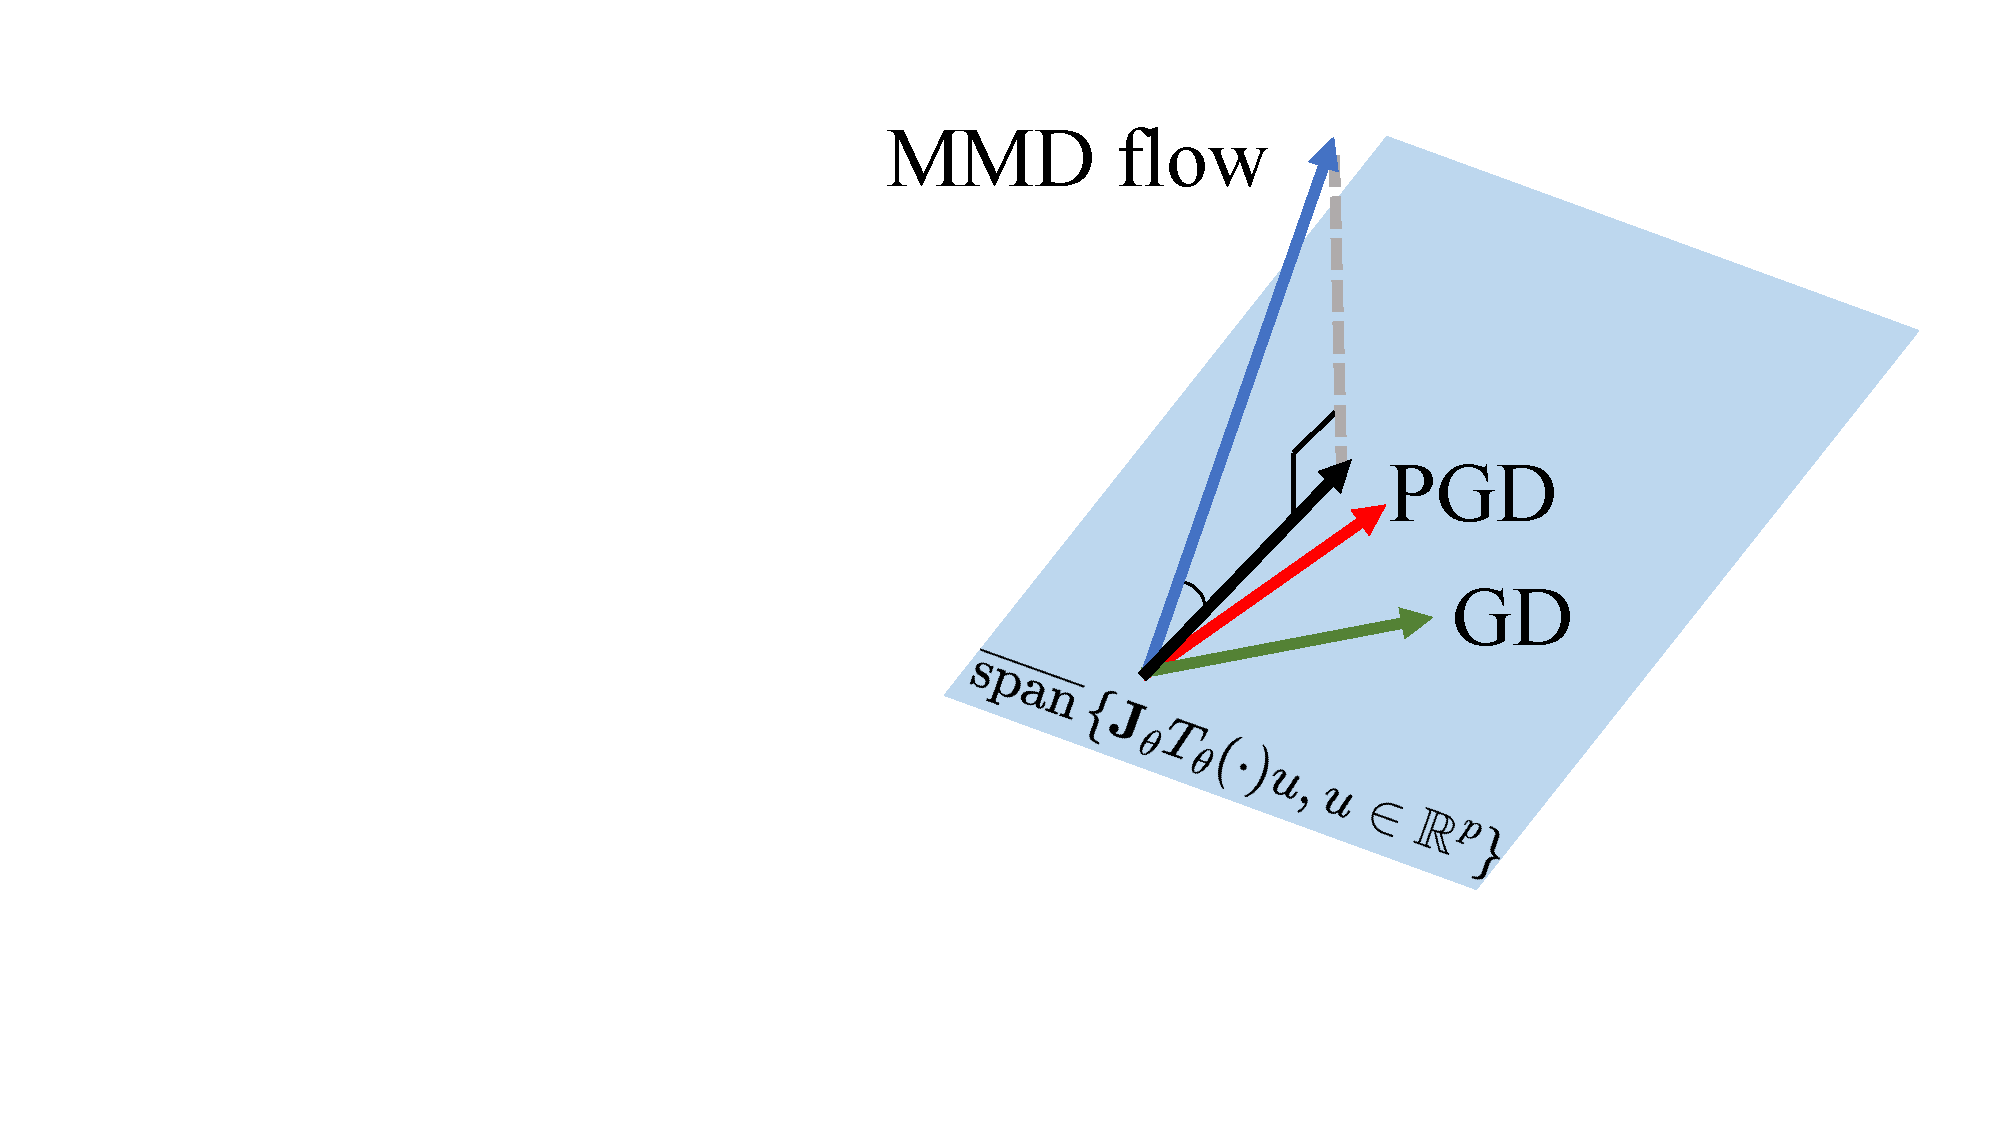
\includegraphics[
                width=\linewidth,
                keepaspectratio
            ]{../plotting/figures/illustration_simple.pdf}
        \end{minipage}
    \end{columns}
\end{frame}


\begin{frame}{Part III: Statistical inference}
    \fcolorbox{mmdBlue!70!black}{mmdBlue!6}{%
    \begin{minipage}[t][0.29\textheight][t]{0.95\linewidth}
        \centering
        {\bfseries On Optimization of Minimum MMD Estimators~\textcolor{mmdBlue!80!black}{(Arxiv)}}\\[-0.10cm]
        {\tiny\textcolor{graytext}{S. S. Kang, L. Sharrock, X. Cheng, F.-X. Briol, \underline{Z. Chen}}}\\[-0.10cm]

        \raggedright
        \begin{itemize}
            \item A preconditioned  method / natural gradient type method. 
            \item Adaptive kernel lengthscale.
        \end{itemize}
    \end{minipage}%
    }
\end{frame}

\parttitleframe{What next: causal inference.}

\begin{frame}{Part IV: What next?}
    \centering
    {\large\bfseries Minimum MMD for counterfactual inference}\\[0.05cm]

    \begin{exampleblock}{}
        \centering
        \textbf{Question:} What would have happened under a different intervention?
    \end{exampleblock}

    \vspace{0cm}
    \begin{block}{}
        \begin{columns}[T,onlytextwidth]
            \column{0.46\textwidth}
            \begin{itemize}
                \setlength\itemsep{0cm}
                \item Treatment $A$. 
                \item Counterfactual outcome: $Y(a)$ under treatment $A=a$.
                \item Missing data/inference problem. 
            \end{itemize}

            \column{0.50\textwidth}
            \centering
            
\includegraphics[width=0.58\linewidth]{figures/counterfactual_inference.png}
        \end{columns}
    \end{block}

    \vspace{0.28cm}
    {\setlength{\fboxsep}{0.30em}%
    \fcolorbox{mmdBlue!70!black}{mmdBlue!5}{%
    \begin{minipage}{0.945\linewidth}
        \raggedright
        {\footnotesize\bfseries Conformal Counterfactual Inference under Hidden Confounding~\textcolor{mmdBlue!80!black}{(KDD 2024)}}\par\vspace{-0.08cm}
        {\tiny\textcolor{graytext}{\underline{Z. Chen}, R. Guo, J.-F. Ton, Y. Liu}}\par\vspace{0.02cm}
        {\footnotesize\bfseries Neural Networks for NPIV: Optimization and Generalization~\textcolor{mmdBlue!80!black}{(Arxiv)}}\par\vspace{-0.08cm}
        {\tiny\textcolor{graytext}{\underline{Z. Chen}, A. Nitanda, A. Gretton, T. Suzuki}}\par\vspace{0.02cm}
        {\footnotesize\bfseries NPIV with Observed Covariates~\textcolor{mmdBlue!80!black}{(Arxiv)}}\par\vspace{-0.08cm}
        {\tiny\textcolor{graytext}{Z. Shen*, \underline{Z. Chen}*, D. Meunier, I. Steinwart, A. Gretton, Z. Li}}
    \end{minipage}}}
\end{frame}

\parttitleframe{Summary}

\begin{frame}{Summary}
    \begin{itemize}
        \item MMD is a powerful tool for comparing probability distributions:
    \begin{align*}
        \text{MMD}(\Pb, \Qb) := \sup_{f \in \calH}
        |\E_{\Pb}[f(X)] - \E_{\Qb}[f(X)]|.
    \end{align*}
        \item Minimization of MMD in ....
    \end{itemize}
    \begin{columns}[T,onlytextwidth]
        \column{0.31\textwidth}
        \centering
        \setlength{\fboxsep}{5pt}
        \fcolorbox{mmdGreen!65!black}{mmdGreen!8}{%
            \begin{minipage}[t][0.35\textheight][t]{0.88\linewidth}
                \centering
                {\Large \mmdicon{mmdGreen!80!black}{$\int$}}\\[0.08cm]
                \begin{minipage}[t][0.70cm][c]{\linewidth}
                    \centering
                    {\bfseries Numerical Integration}
                \end{minipage}\\[0.08cm]
                \begin{minipage}[t][1.18cm][c]{\linewidth}
                    \centering
                    {\small$
                    \begin{gathered}
                    \min_{w_{1:n}\in\R^n}
                    \mmd\left(\sum_{i=1}^n w_i \delta_{x_i}, \Pb\right)
                    \end{gathered}$}
                \end{minipage}
            \end{minipage}
        }
        \column{0.31\textwidth}
        \centering
        \setlength{\fboxsep}{5pt}
        \fcolorbox{mmdBlue!70!black}{mmdBlue!8}{%
            \begin{minipage}[t][0.35\textheight][t]{0.88\linewidth}
                \centering
                {\Large \mmdicon{mmdBlue!80!black}{$\sim$}}\\[0.08cm]
                \begin{minipage}[t][0.70cm][c]{\linewidth}
                    \centering
                    {\bfseries Sampling / generative modelling}
                \end{minipage}\\[0.08cm]
                \begin{minipage}[t][1.18cm][c]{\linewidth}
                    \centering
                    {\small$
                    \min_{\Pb \in \calP(\R^d)}
                    \mmd^2(\Pb, \Qb)$}
                \end{minipage}
            \end{minipage}
        }

        \column{0.31\textwidth}
        \centering
        \setlength{\fboxsep}{5pt}
        \fcolorbox{mmdRed!70!black}{mmdRed!8}{%
            \begin{minipage}[t][0.35\textheight][t]{0.88\linewidth}
                \centering
                {\Large \mmdicon{mmdRed!80!black}{$\theta$}}\\[0.08cm]
                \begin{minipage}[t][0.70cm][c]{\linewidth}
                    \centering
                    {\bfseries Statistical inference}
                \end{minipage}\\[0.08cm]
                \begin{minipage}[t][1.18cm][c]{\linewidth}
                    \centering
                    {\small$
                    \min_{\theta \in \Theta}
                    \mathrm{MMD}^2(\Pb_\theta,\Qb)$}
                \end{minipage}
            \end{minipage}
        }
    \end{columns}


\end{frame}

\bibliographystyle{alpha}
\bibliography{reference}

\end{document}
